\chapter{Accuracy of the Multi-Bit Spike Train Model}
\label{appendix:accuracy}

\section{Accuracy Curves}
\label{appendix:accuracy_curves}

    All train accuracy curves are smoothed with a window size of 100.

    The hyperparameters used in the training process are shown in Table \ref{tab:hyperparameters_accuracy}.

    \begin{table}[H]
        \begin{tabularx}{\textwidth}{|X|c|c|c|c|c|c|c|}
            \toprule
            Dataset & Reps & Epochs & LR & Opt & Batch & Time steps \\
            \midrule
            Fashion MNIST & 10 & 5 & 2e-3 & Adam & 128 & 10 \\
            MNIST & 10 & 5 & 2e-3 & Adam & 128 & 10 \\
            NMNIST & 10 & 5 & 2e-3 & Adam & 128 & 10 \\
            DVS Gesture & 10 & 20 & 1e-3 & Adam & 128 & 10 \\
            CIFAR-10 & 5 & 50 & 1e-5 & Adam & 128 & 10 \\
            \bottomrule
        \end{tabularx}
        \caption{Hyperparameters}
        \label{tab:hyperparameters_accuracy}
    \end{table}

    \label{appendix:accuracy_curves_fashion_mnist}
        \begin{figure}[H]
            \centering
            \begin{subfigure}[H]{0.55\textwidth}
                \centering
                \begin{subfigure}[H]{\textwidth}
                    \centering
                    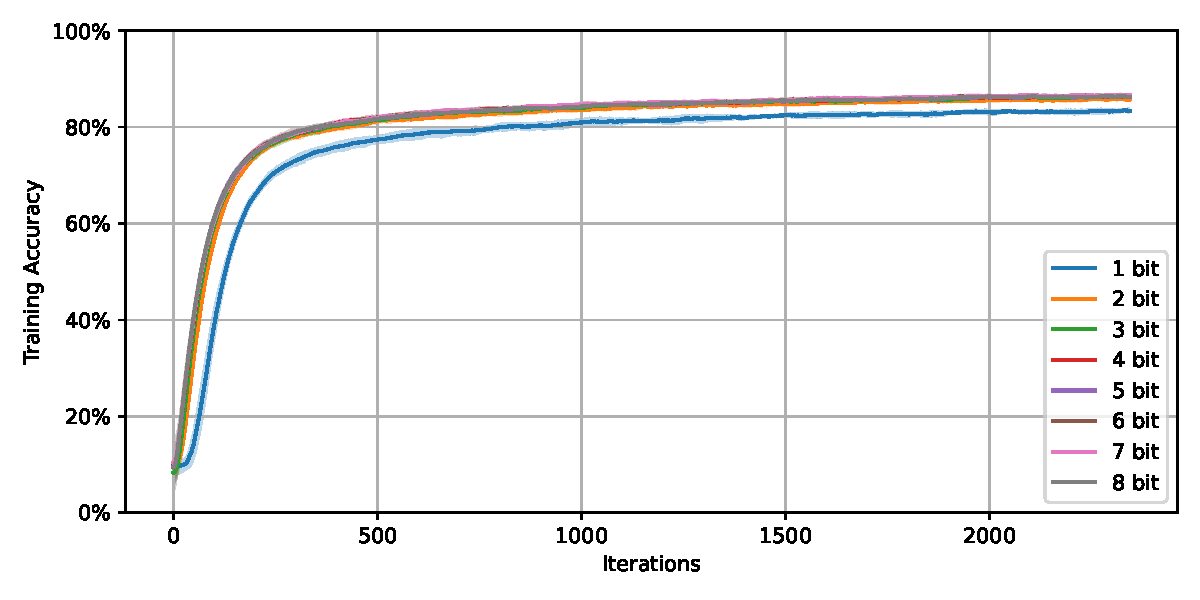
\includegraphics[width=\textwidth]{../standard/FashionMNIST/plots/fashionmnist_train_acc.pdf}
                    \caption{Train Accuracy}
                \end{subfigure}
                \hfill
                \begin{subfigure}[H]{\textwidth}
                    \centering
                    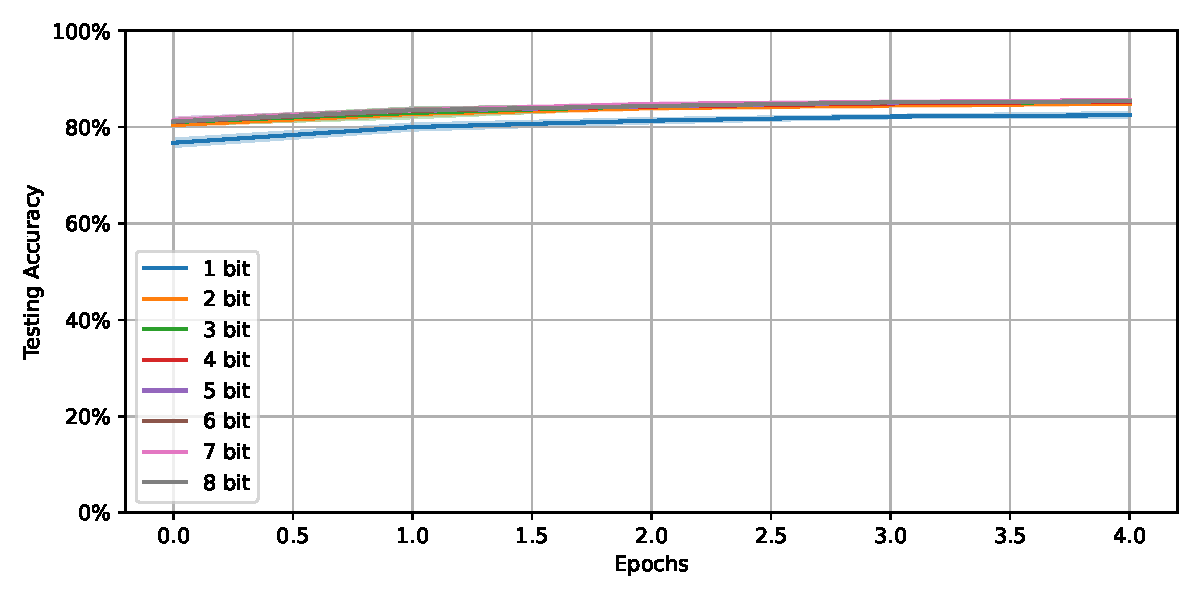
\includegraphics[width=\textwidth]{../standard/FashionMNIST/plots/fashionmnist_test_acc.pdf}
                    \caption{Test Accuracy}
                \end{subfigure}
            \end{subfigure}
            \hfill
            \begin{subfigure}[H]{0.3\textwidth}
                \centering
                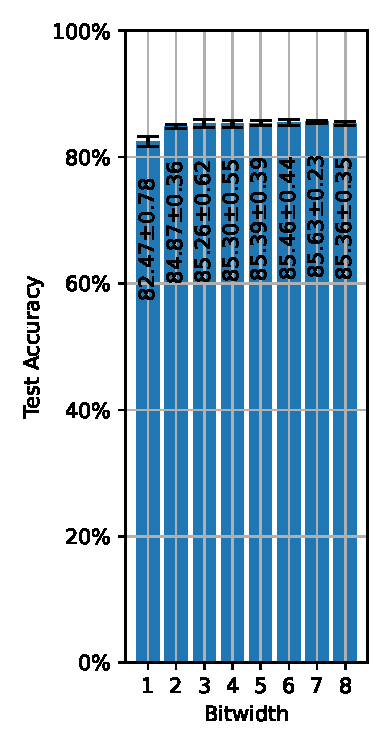
\includegraphics[width=\textwidth]{../standard/FashionMNIST/plots/fashionmnist_final_acc.pdf}
                \caption{Final Test Accuracy}
            \end{subfigure}
            \caption{Accuracy Curves of the Fashion MNIST Model}
        \end{figure}

    \label{appendix:accuracy_curves_mnist}
        \begin{figure}[H]
            \centering
            \begin{subfigure}[H]{0.55\textwidth}
                \centering
                \begin{subfigure}[H]{\textwidth}
                    \centering
                    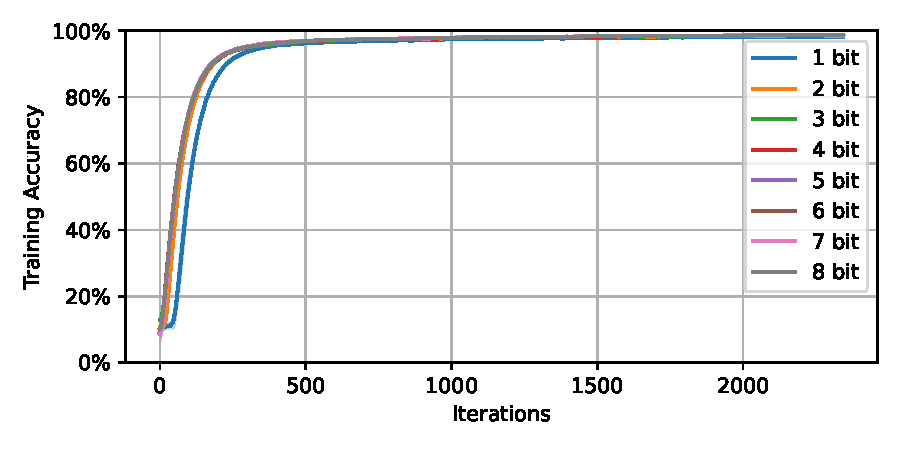
\includegraphics[width=\textwidth]{../standard/MNIST/plots/mnist_train_acc.pdf}
                    \caption{Train Accuracy}
                \end{subfigure}
                \hfill
                \begin{subfigure}[H]{\textwidth}
                    \centering
                    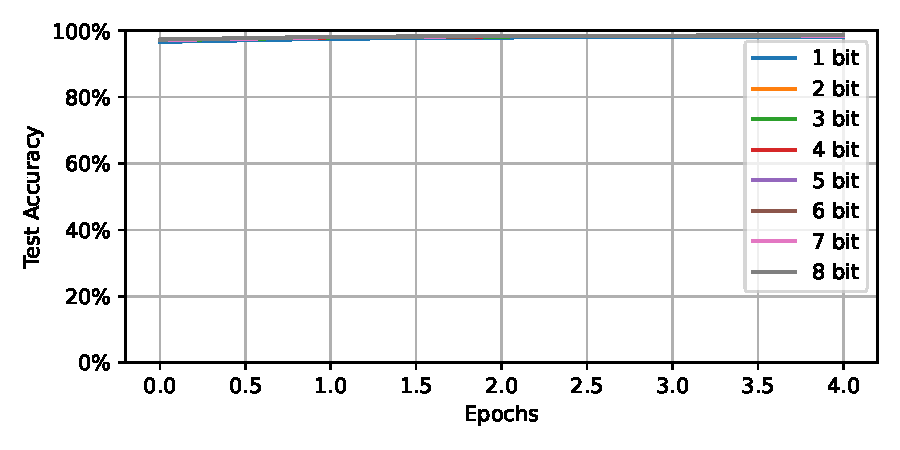
\includegraphics[width=\textwidth]{../standard/MNIST/plots/mnist_test_acc.pdf}
                    \caption{Test Accuracy}
                \end{subfigure}
            \end{subfigure}
            \hfill
            \begin{subfigure}[H]{0.3\textwidth}
                \centering
                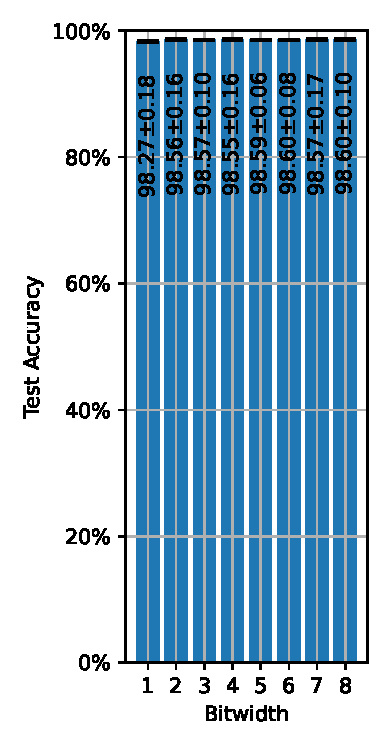
\includegraphics[width=\textwidth]{../standard/MNIST/plots/mnist_final_acc.pdf}
                \caption{Final Test Accuracy}
            \end{subfigure}
            \caption{Accuracy Curves of the MNIST Model}
        \end{figure}
    
    \label{appendix:accuracy_curves_nmnist}
        \begin{figure}[H]
            \centering
            \begin{subfigure}[H]{0.55\textwidth}
                \centering
                \begin{subfigure}[H]{\textwidth}
                    \centering
                    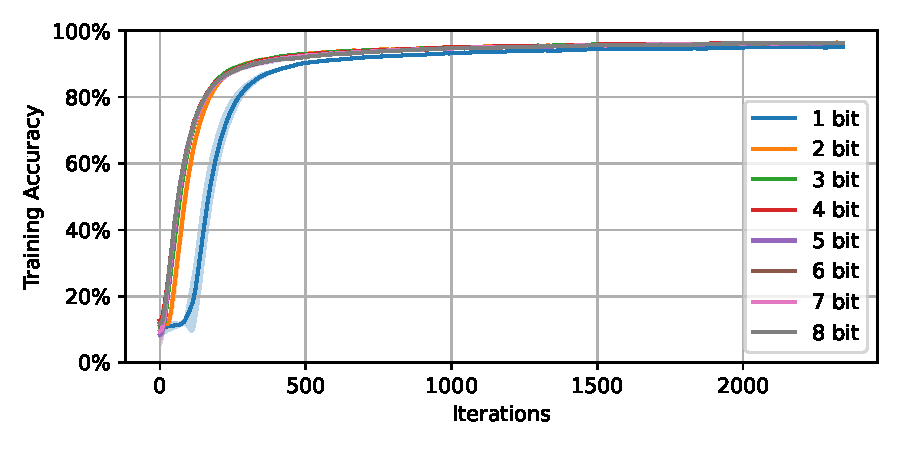
\includegraphics[width=\textwidth]{../standard/NMNIST/plots/nmnist_train_acc.pdf}
                    \caption{Train Accuracy}
                \end{subfigure}
                \hfill
                \begin{subfigure}[H]{\textwidth}
                    \centering
                    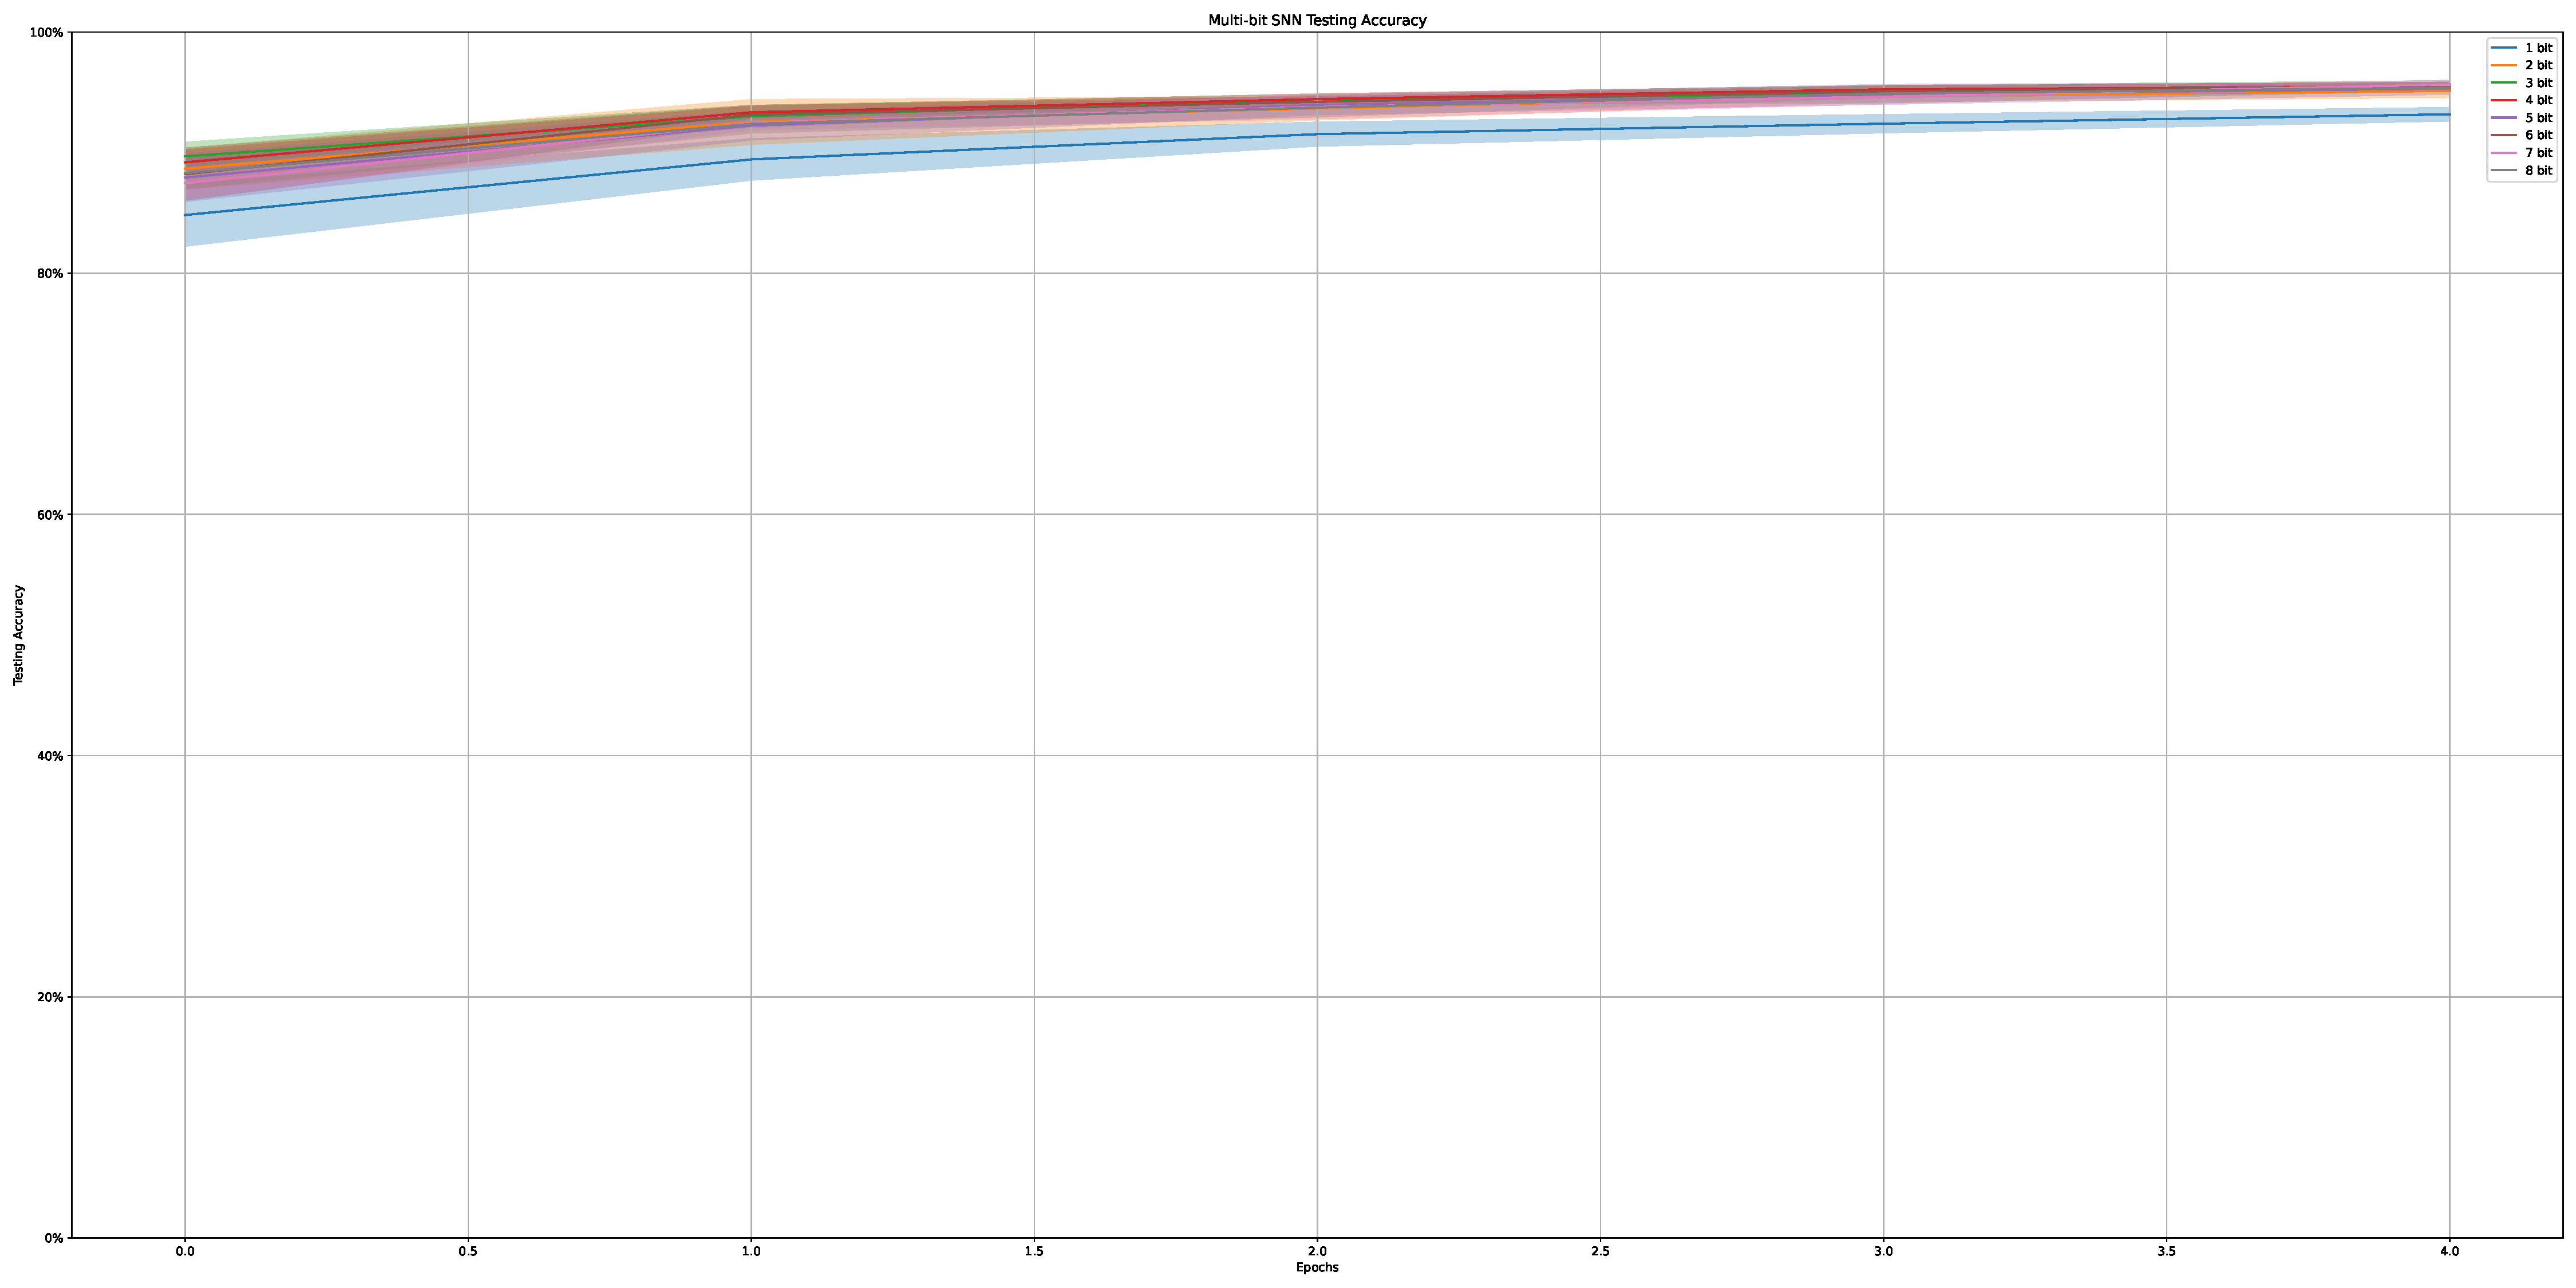
\includegraphics[width=\textwidth]{../standard/NMNIST/plots/nmnist_test_acc.pdf}
                    \caption{Test Accuracy}
                \end{subfigure}
            \end{subfigure}
            \hfill
            \begin{subfigure}[H]{0.3\textwidth}
                \centering
                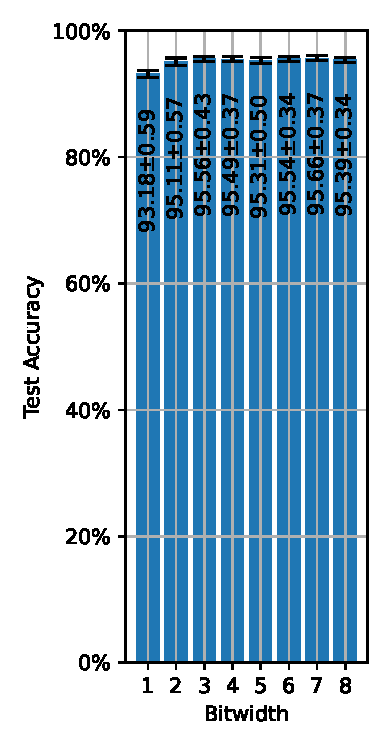
\includegraphics[width=\textwidth]{../standard/NMNIST/plots/nmnist_final_acc.pdf}
                \caption{Final Test Accuracy}
            \end{subfigure}
            \caption{Accuracy Curves of the NMNIST Model}
        \end{figure}

    \label{appendix:accuracy_curves_dvs_gesture}
        \begin{figure}[H]
            \centering
            \begin{subfigure}[H]{0.55\textwidth}
                \centering
                \begin{subfigure}[H]{\textwidth}
                    \centering
                    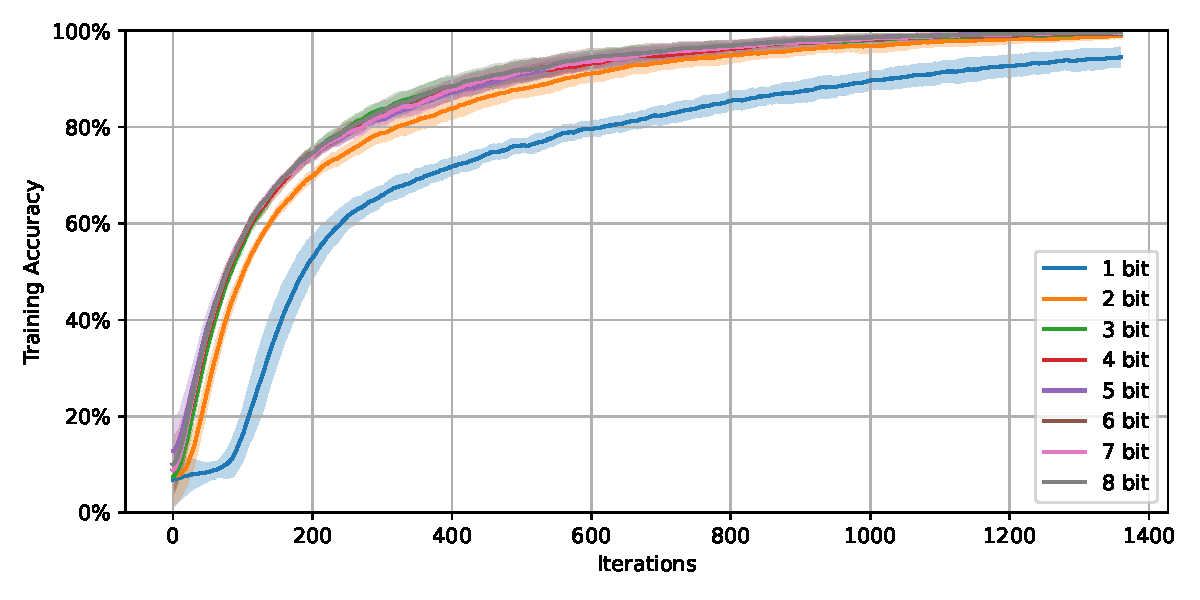
\includegraphics[width=\textwidth]{../standard/DVSGesture/plots/dvsgesture_train_acc.pdf}
                    \caption{Train Accuracy}
                \end{subfigure}
                \hfill
                \begin{subfigure}[H]{\textwidth}
                    \centering
                    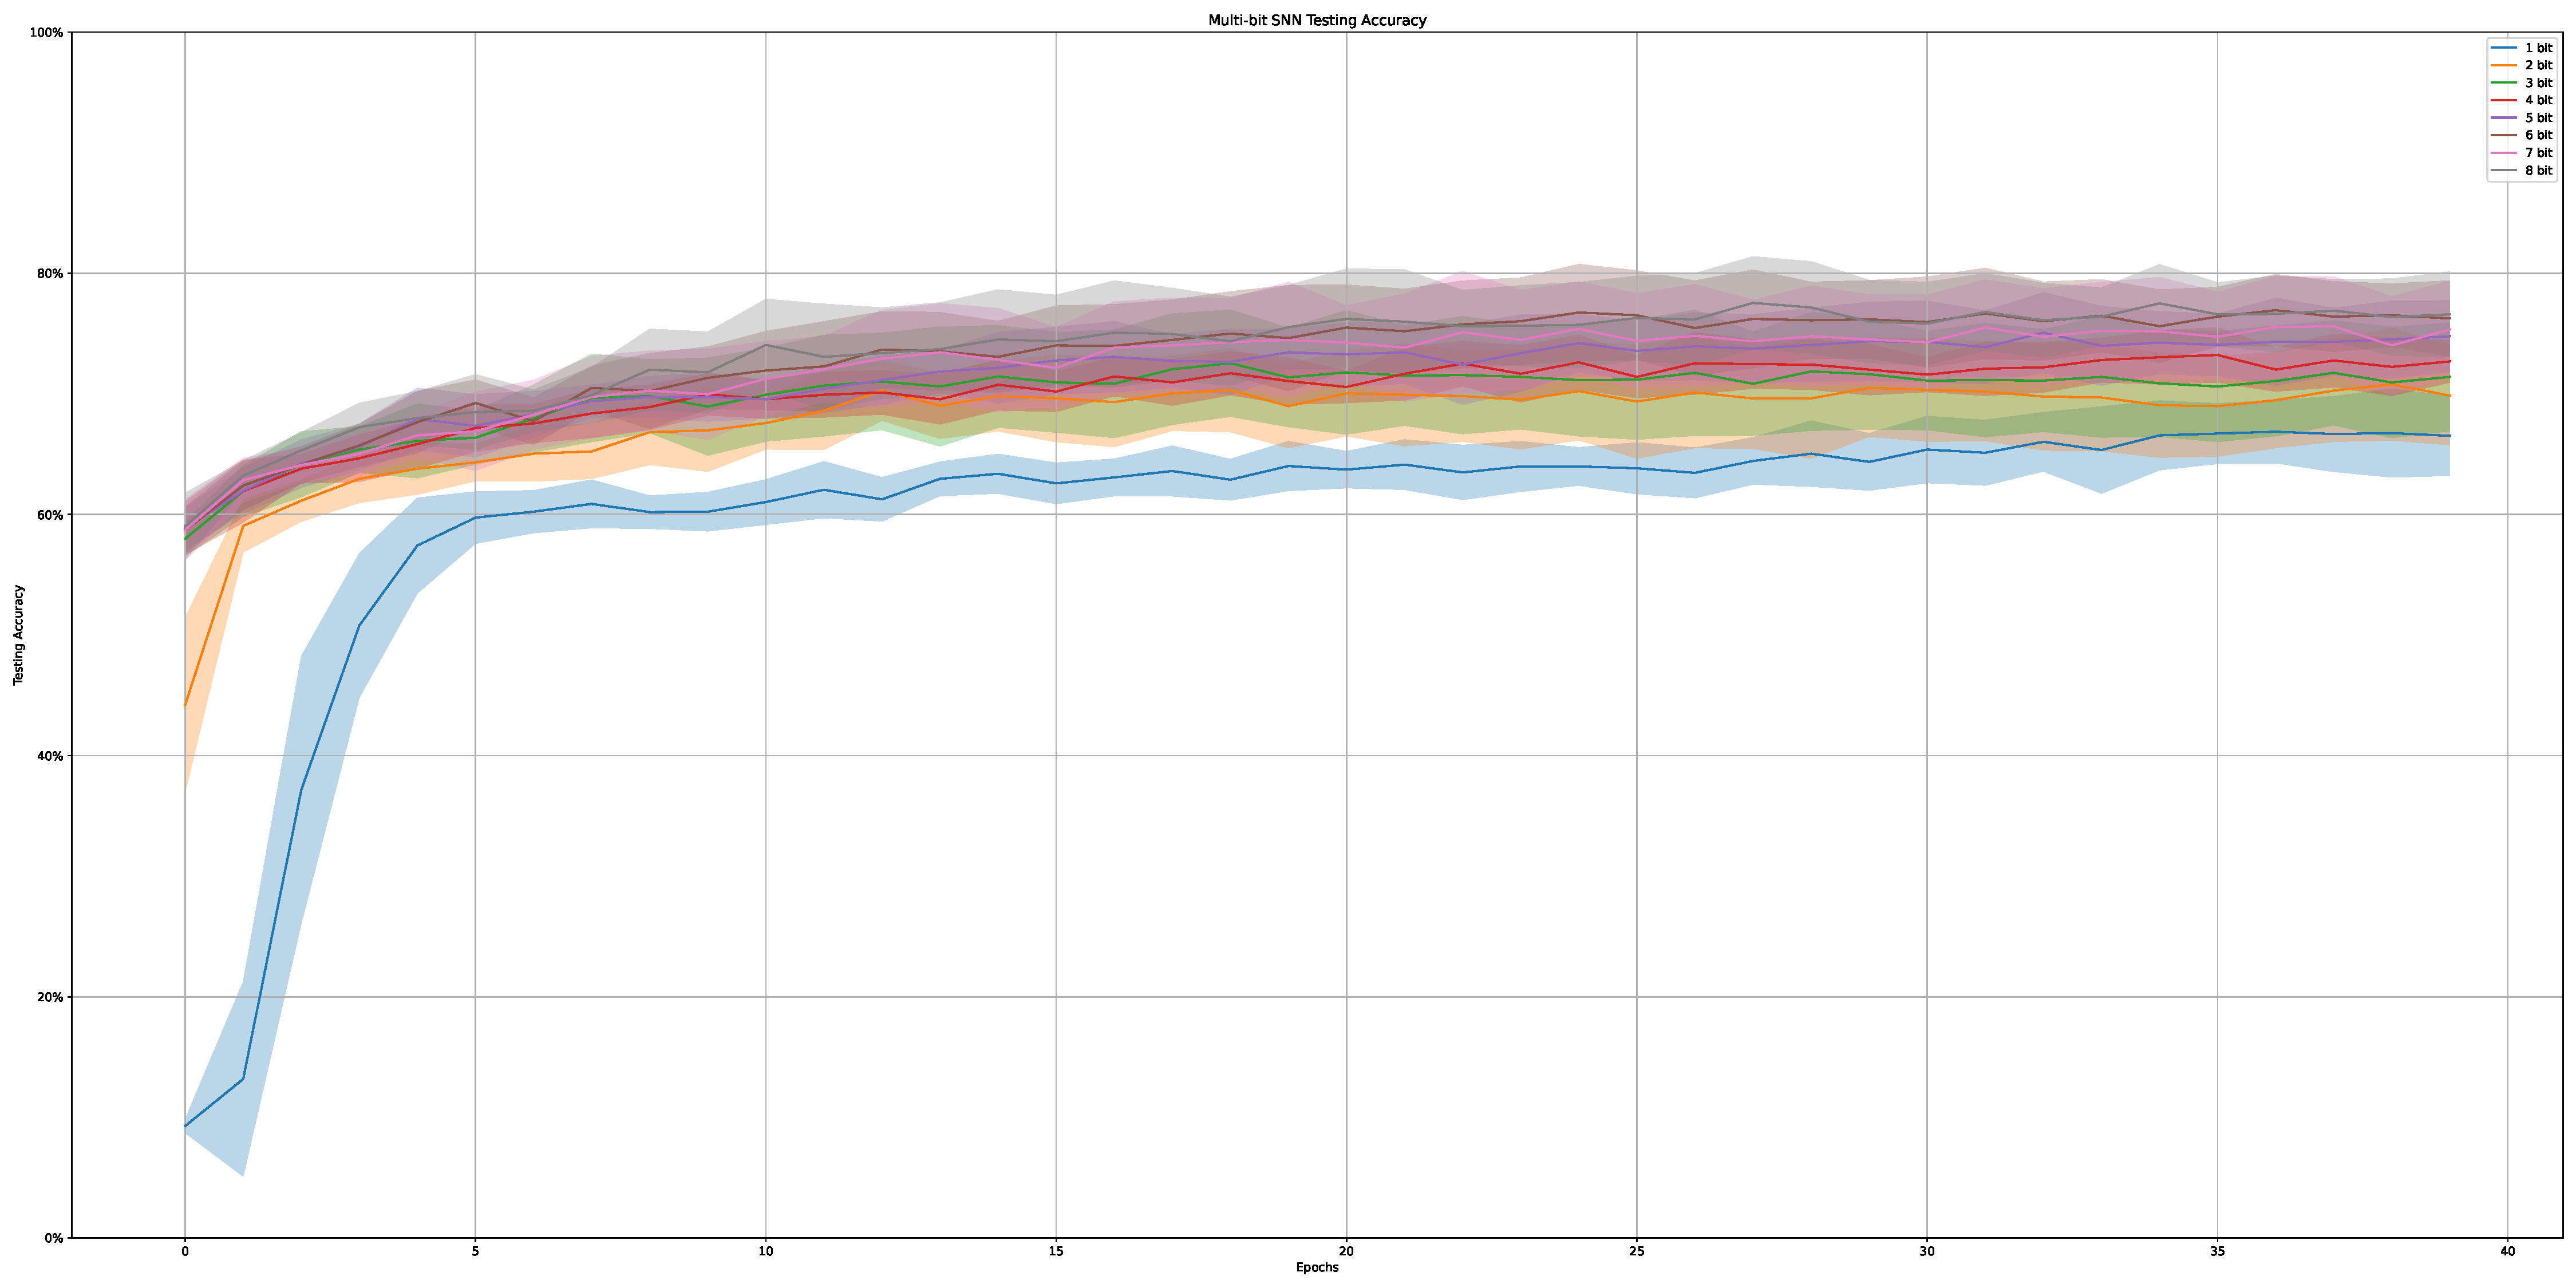
\includegraphics[width=\textwidth]{../standard/DVSGesture/plots/dvsgesture_test_acc.pdf}
                    \caption{Test Accuracy}
                \end{subfigure}
            \end{subfigure}
            \hfill
            \begin{subfigure}[H]{0.3\textwidth}
                \centering
                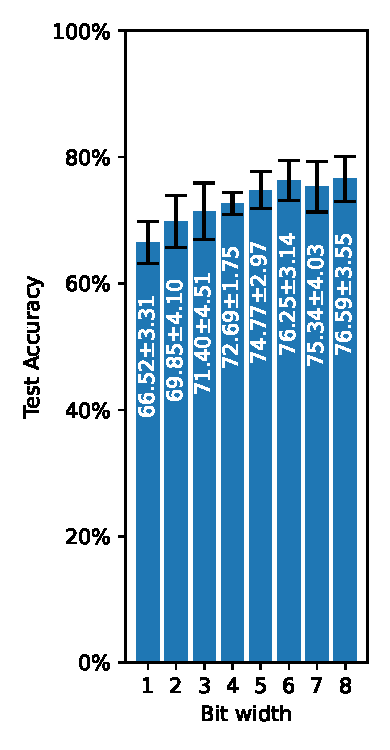
\includegraphics[width=\textwidth]{../standard/DVSGesture/plots/dvsgesture_final_acc.pdf}
                \caption{Final Test Accuracy}
            \end{subfigure}
            \caption{Accuracy Curves of the DVS Gesture Model}
        \end{figure}

    \label{appendix:accuracy_curves_cifar10}
        \begin{figure}[H]
            \centering
            \begin{subfigure}[H]{0.55\textwidth}
                \centering
                \begin{subfigure}[H]{\textwidth}
                    \centering
                    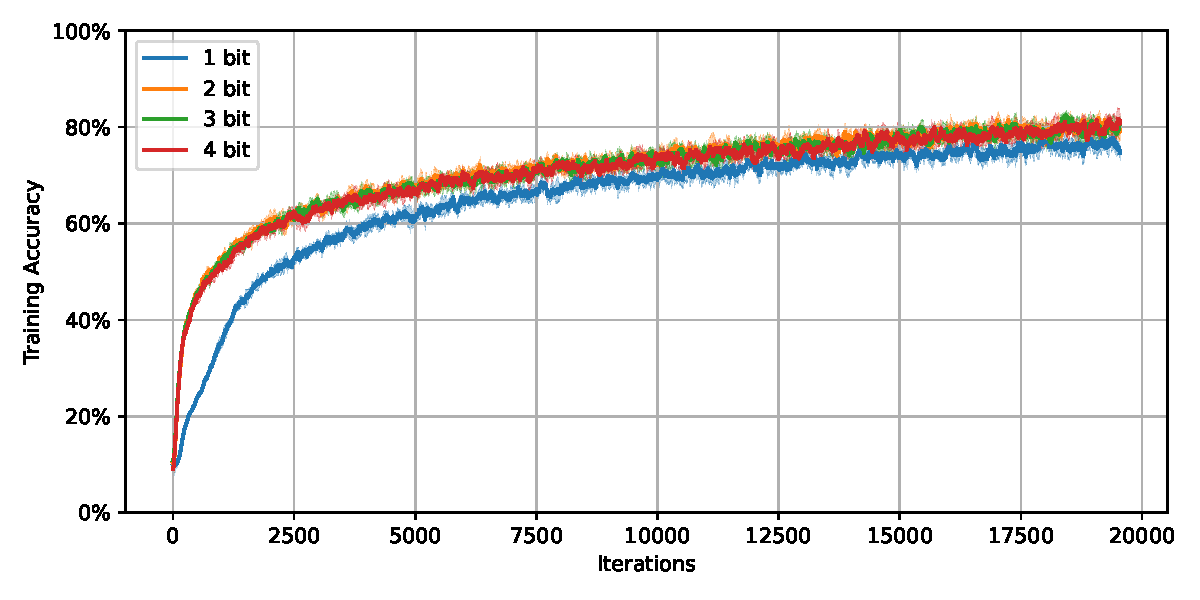
\includegraphics[width=\textwidth]{../standard/CIFAR10/plots/cifar10_train_acc.pdf}
                    \caption{Train Accuracy}
                \end{subfigure}
                \hfill
                \begin{subfigure}[H]{\textwidth}
                    \centering
                    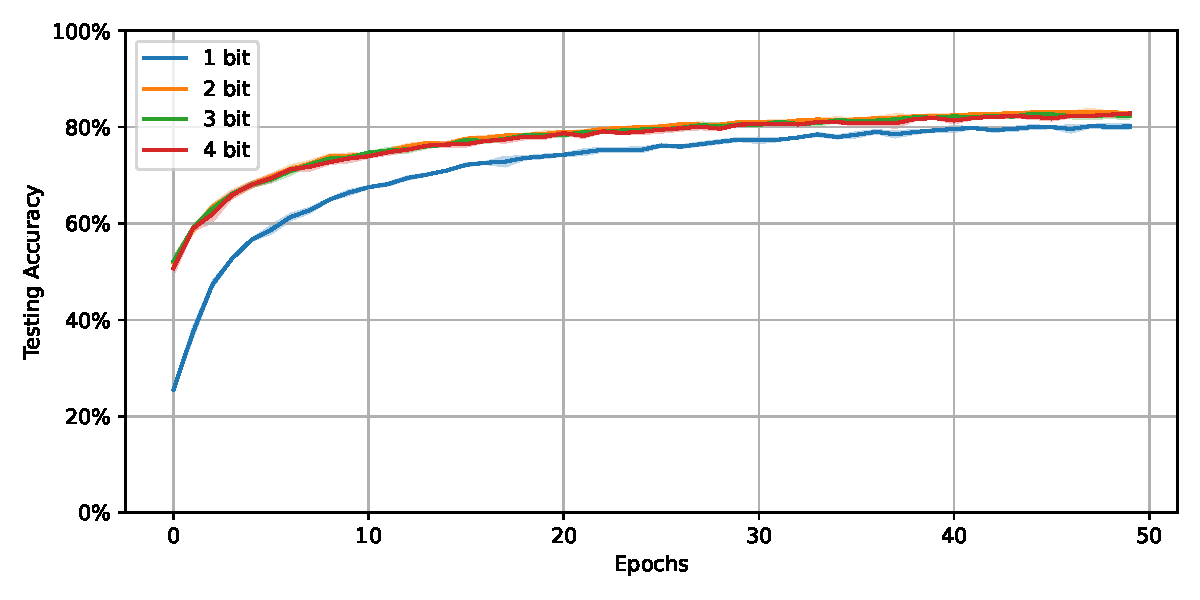
\includegraphics[width=\textwidth]{../standard/CIFAR10/plots/cifar10_test_acc.pdf}
                    \caption{Test Accuracy}
                \end{subfigure}
            \end{subfigure}
            \hfill
            \begin{subfigure}[H]{0.3\textwidth}
                \centering
                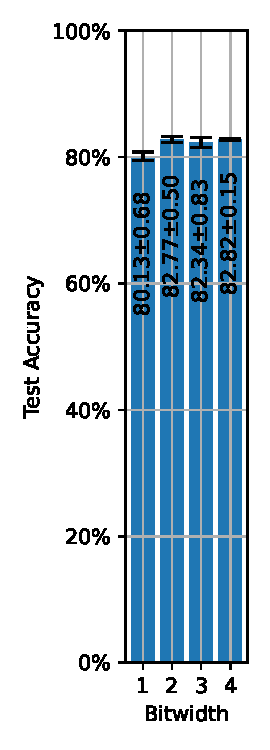
\includegraphics[width=\textwidth]{../standard/CIFAR10/plots/cifar10_final_acc.pdf}
                \caption{Final Test Accuracy}
            \end{subfigure}
            \caption{Accuracy Curves of the CIFAR-10 Model}
        \end{figure}

\section{Iterations and Epochs to Reach the Target Accuracy}
\label{appendix:iterations}
    In this section, we consider the target accuracy to be 80\%. 

    Hyperparameters: Same as in Table \ref{tab:hyperparameters_accuracy}.

    \label{appendix:iterations_fashion_mnist}
        \begin{figure}[H]
            \centering
            \begin{subfigure}[H]{0.6\textwidth}
                \centering
                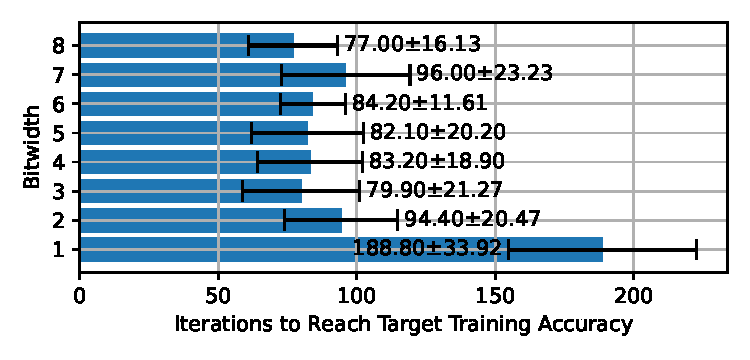
\includegraphics[width=\textwidth]{../standard/FashionMNIST/plots/fashionmnist_train_iters_horizontal.pdf}
                \caption{Iterations to Reach the Training Accuracy}
            \end{subfigure}
        \end{figure}
        \begin{figure}[H]
            \centering
            \ContinuedFloat
            \begin{subfigure}[H]{0.6\textwidth}
                \centering
                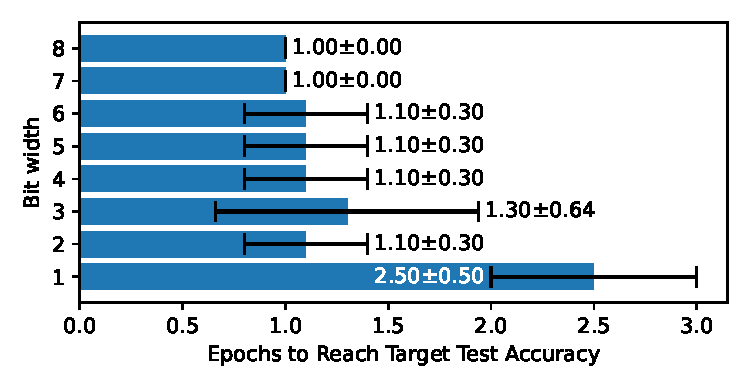
\includegraphics[width=\textwidth]{../standard/FashionMNIST/plots/fashionmnist_test_iters_horizontal.pdf}
                \caption{Epochs to Reach the Test Accuracy}
            \end{subfigure}
            \caption{Required Iterations of Epochs on Fashion MNIST}
        \end{figure}

    \label{appendix:iterations_mnist}
        \begin{figure}[H]
            \centering
            \begin{subfigure}[H]{0.6\textwidth}
                \centering
                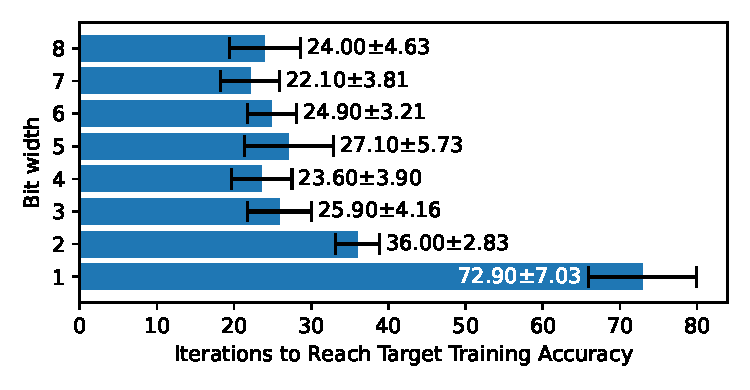
\includegraphics[width=\textwidth]{../standard/MNIST/plots/mnist_train_iters_horizontal.pdf}
                \caption{Iterations to Reach the Training Accuracy}
            \end{subfigure}
        \end{figure}
        \begin{figure}[H]
            \centering
            \ContinuedFloat
            \begin{subfigure}[H]{0.6\textwidth}
                \centering
                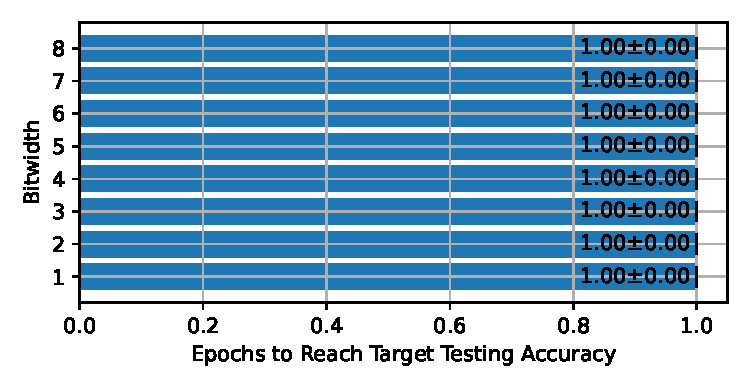
\includegraphics[width=\textwidth]{../standard/MNIST/plots/mnist_test_iters_horizontal.pdf}
                \caption{Epochs to Reach the Test Accuracy}
            \end{subfigure}
            \caption{Required Iterations of Epochs on MNIST}
        \end{figure}

    \label{appendix:iterations_nmnist}
        \begin{figure}[H]
            \centering
            \begin{subfigure}[H]{0.6\textwidth}
                \centering
                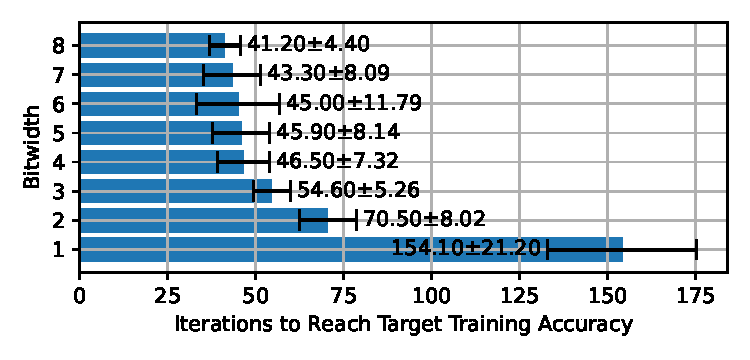
\includegraphics[width=\textwidth]{../standard/NMNIST/plots/nmnist_train_iters_horizontal.pdf}
                \caption{Iterations to Reach the Training Accuracy}
            \end{subfigure}
        \end{figure}
        \begin{figure}[H]
            \centering
            \ContinuedFloat
            \begin{subfigure}[H]{0.6\textwidth}
                \centering
                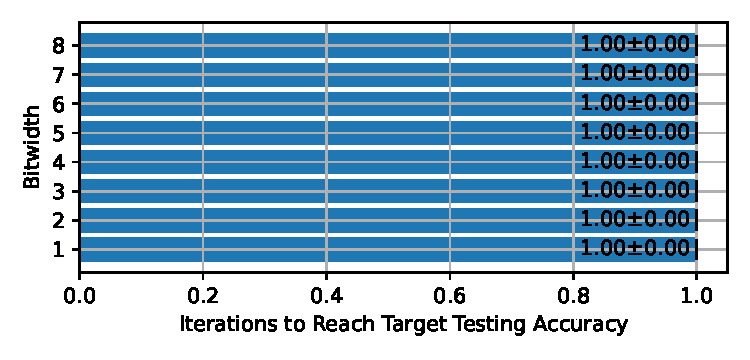
\includegraphics[width=\textwidth]{../standard/NMNIST/plots/nmnist_test_iters_horizontal.pdf}
                \caption{Epochs to Reach the Test Accuracy}
            \end{subfigure}
            \caption{Required Iterations of Epochs on NMNIST}
        \end{figure}

    \label{appendix:iterations_dvs_gesture}
        \begin{figure}[H]
            \centering
            \begin{subfigure}[H]{0.6\textwidth}
                \centering
                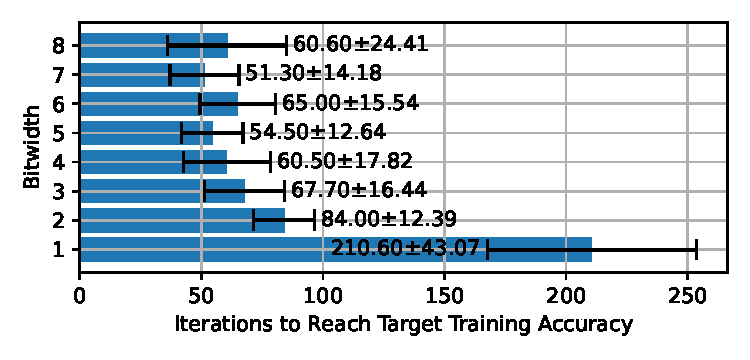
\includegraphics[width=\textwidth]{../standard/DVSGesture/plots/dvsgesture_train_iters_horizontal.pdf}
                \caption{Iterations to Reach the Training Accuracy}
            \end{subfigure}
        \end{figure}
        \begin{figure}[H]
            \centering
            \ContinuedFloat
            \begin{subfigure}[H]{0.6\textwidth}
                \centering
                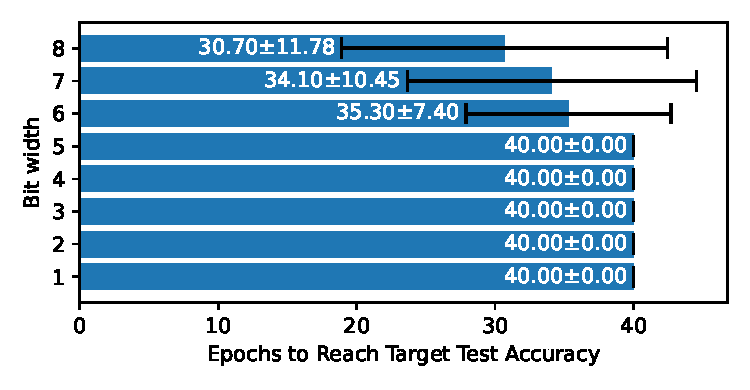
\includegraphics[width=\textwidth]{../standard/DVSGesture/plots/dvsgesture_test_iters_horizontal.pdf}
                \caption{Epochs to Reach the Test Accuracy}
            \end{subfigure}
            \caption{Required Iterations of Epochs on DVS Gesture}
        \end{figure}

    Notice that we encountered overfitting in the DVS Gesture dataset, which is why the number of iterations to reach the target test accuracy is capped at 40 epochs (the maximum number of epochs in the training process), thus not representative. 

    \label{appendix:iterations_cifar10}
        \begin{figure}[H]
            \centering
            \begin{subfigure}[H]{0.6\textwidth}
                \centering
                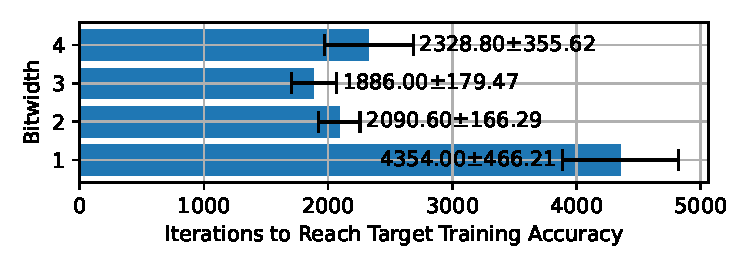
\includegraphics[width=\textwidth]{../standard/CIFAR10/plots/cifar10_train_iters_horizontal.pdf}
                \caption{Iterations to Reach the Training Accuracy}
            \end{subfigure}
        \end{figure}
        \begin{figure}[H]
            \centering
            \ContinuedFloat
            \begin{subfigure}[H]{0.6\textwidth}
                \centering
                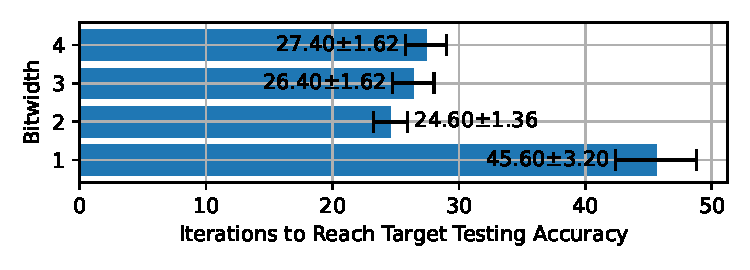
\includegraphics[width=\textwidth]{../standard/CIFAR10/plots/cifar10_test_iters_horizontal.pdf}
                \caption{Epochs to Reach the Test Accuracy}
            \end{subfigure}
            \caption{Required Iterations of Epochs on CIFAR-10}
        \end{figure}



\chapter{Firing Rate in Different Positions of the Multi-Bit Spike Train Model}
\label{appendix:firerate}

    For the ease of debugging, the first measuring position is always just the input data. If the data is captured by a dynamic vision sensor or it is encoded with a Poisson spike generator, one should see a firing rate much below 100\%. In the case of original data (e.g. CIFAR-10), the firing rate should be close to 100\%. 

    From the second measuring position to the last position, the firing rate is measured after the LIF neuron layers. Not all LIF neuron layers are measured. But the last LIF neuron layer is always measured. 

    The hyperparameters used in the training process are shown in Table \ref{tab:hyperparameters_firerate}.

    \begin{table}
        \begin{tabularx}{\textwidth}{|X|c|c|c|c|c|c|c|}
            \toprule
            Dataset & Reps & Epochs & LR & Opt & Batch & Time steps \\
            \midrule
            Fashion MNIST & 10 & 50 & 2e-3 & Adam & 128 & 10 \\
            MNIST & 10 & 50 & 2e-3 & Adam & 128 & 10 \\
            NMNIST & 10 & 50 & 2e-3 & Adam & 128 & 10 \\
            DVS Gesture & 10 & 200 & 1e-3 & Adam & 128 & 10 \\
            CIFAR-10 & 5 & 1000 & 1e-5 & Adam & 128 & 10 \\
            \bottomrule
        \end{tabularx}
        \caption{Hyperparameters}
        \label{tab:hyperparameters_firerate}
    \end{table}

    \section{Fashion MNIST}
    \label{appendix:firerate_fashion_mnist}
        \begin{figure}[H]
            \centering
            \begin{subfigure}[H]{0.8\textwidth}
                \centering
                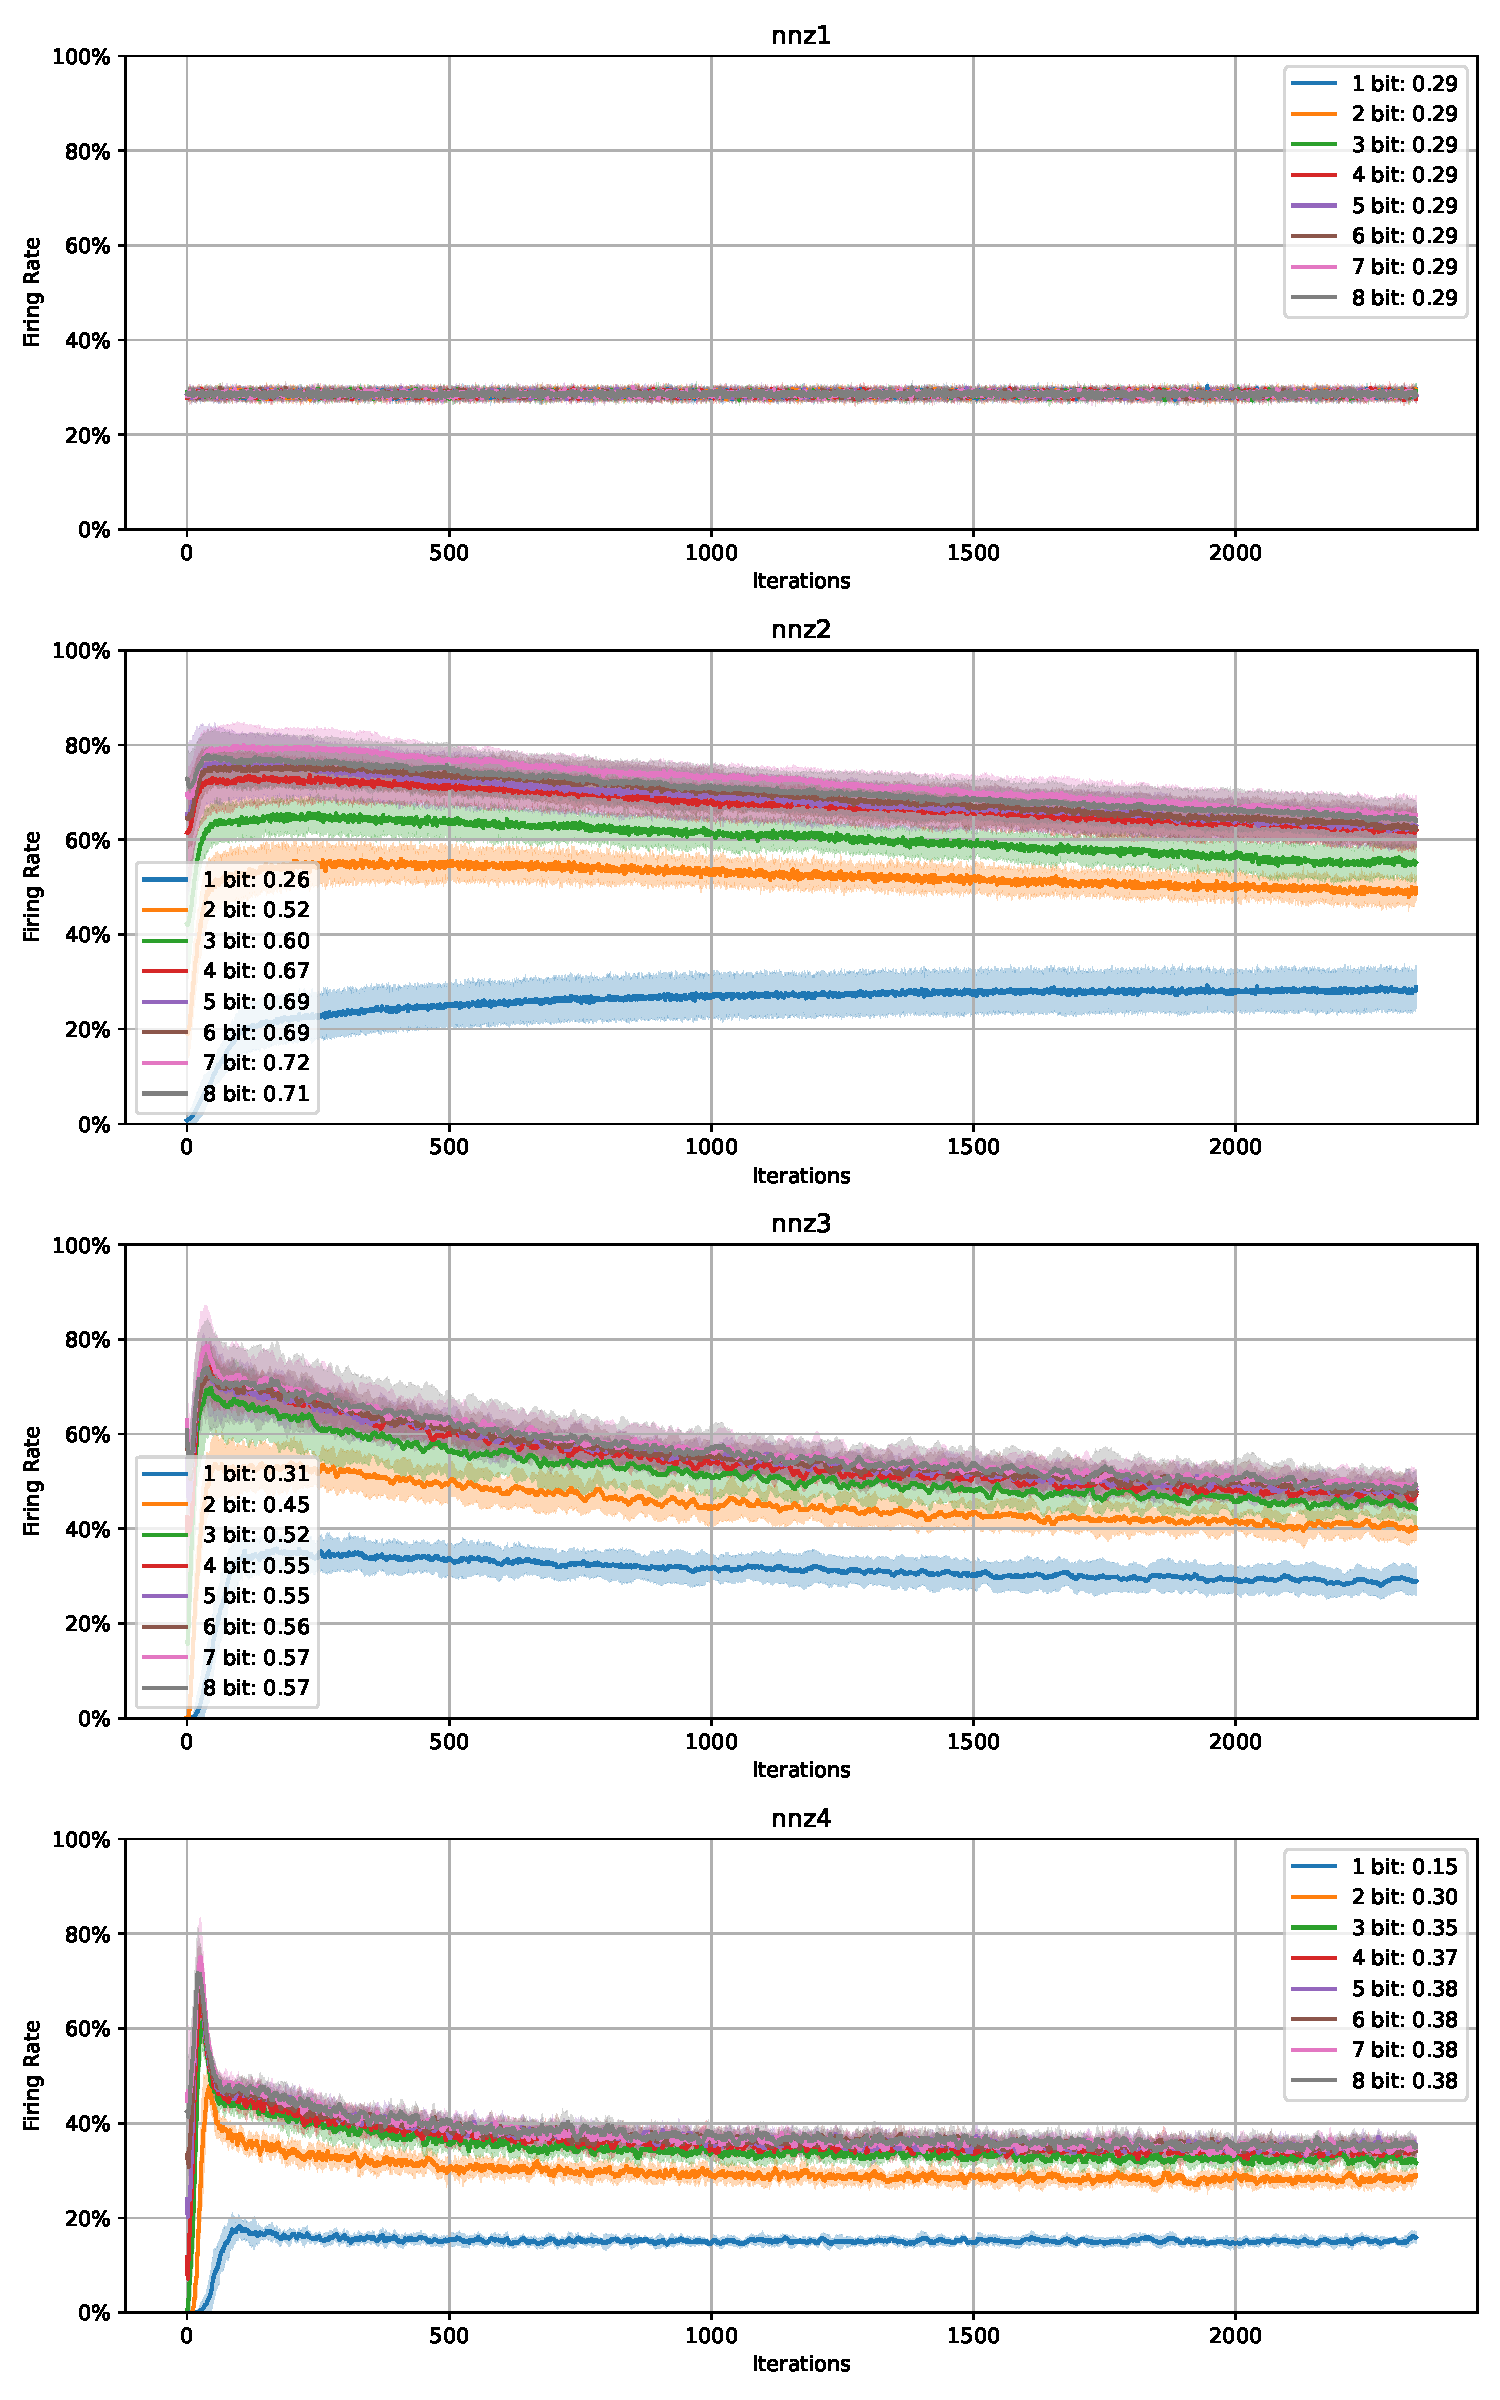
\includegraphics[width=\textwidth]{../firerate/FashionMNIST/plots/fashionmnist_train_firerate.pdf}
                \caption{Firing Rate in Different Positions (Training)}
            \end{subfigure}
        \end{figure}
        \begin{figure}[H]
            \centering
            \ContinuedFloat
            \begin{subfigure}[H]{0.8\textwidth}
                \centering
                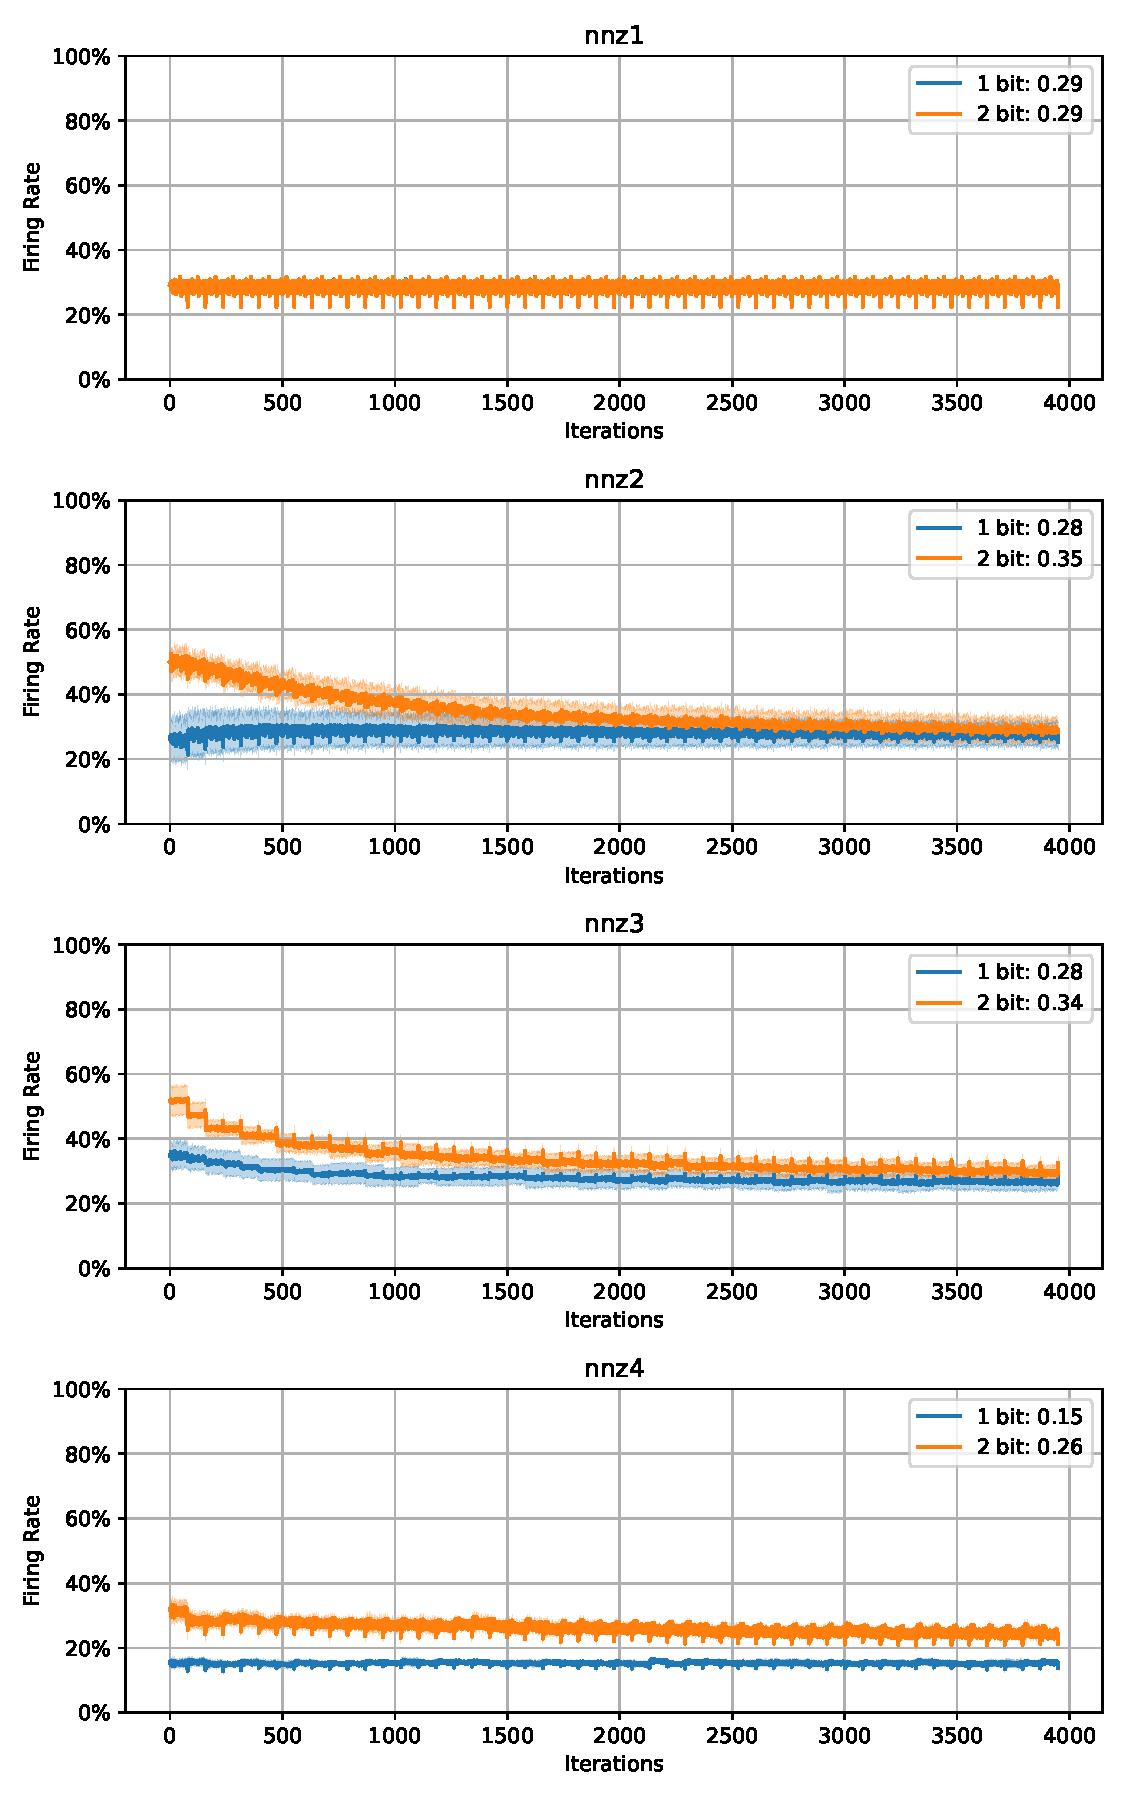
\includegraphics[width=\textwidth]{../firerate/FashionMNIST/plots/fashionmnist_test_firerate.pdf}
                \caption{Firing Rate in Different Positions (Test)}
            \end{subfigure}
        \end{figure}
        \begin{figure}[H]
            \centering
            \ContinuedFloat
            \begin{subfigure}[H]{\textwidth}
                \centering
                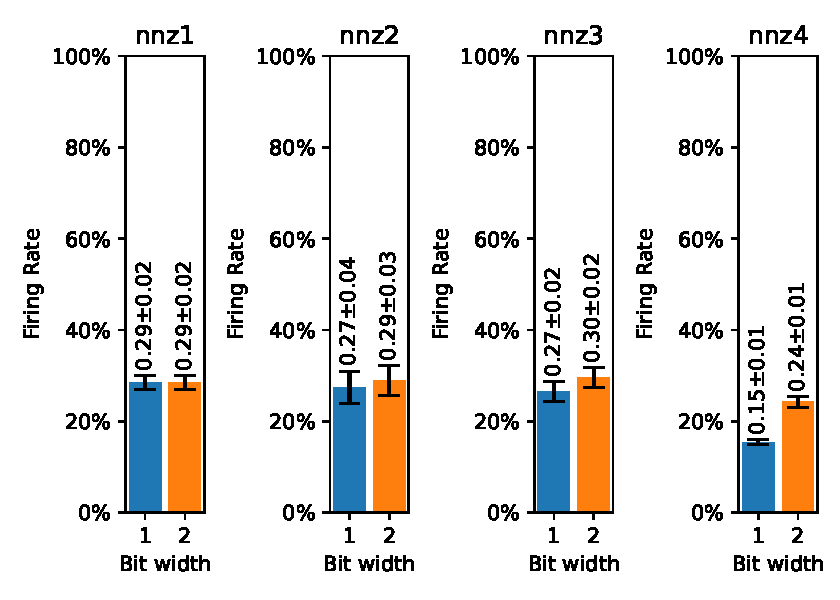
\includegraphics[width=\textwidth]{../firerate/FashionMNIST/plots/fashionmnist_final_firerate.pdf}
                \caption{Firing Rate in Different Positions (Final Test)}
            \end{subfigure}
            \caption{Firing Rate in Different Positions of the Fashion MNIST Model}
        \end{figure}

    \section{MNIST}
    \label{appendix:firerate_mnist}
        \begin{figure}[H]
            \centering
            \begin{subfigure}[H]{0.8\textwidth}
                \centering
                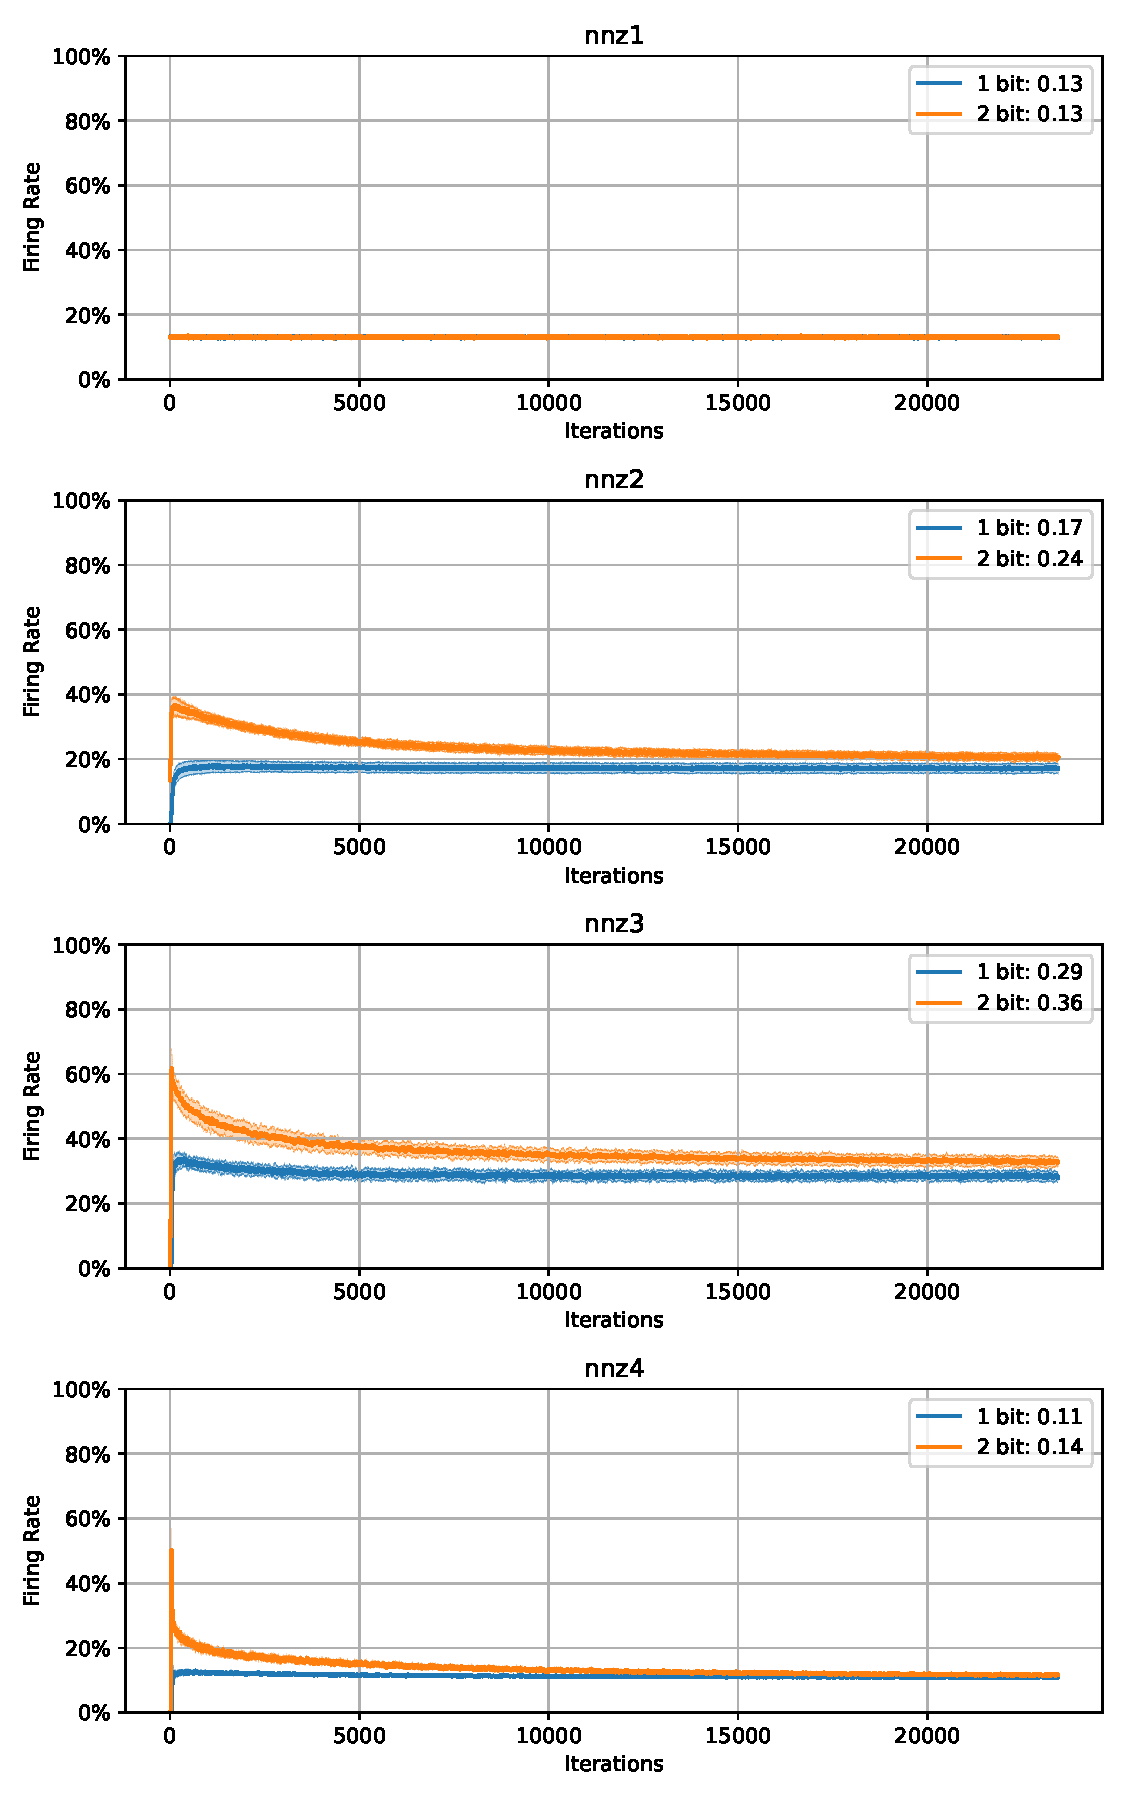
\includegraphics[width=\textwidth]{../firerate/MNIST/plots/mnist_train_firerate.pdf}
                \caption{Firing Rate in Different Positions (Training)}
            \end{subfigure}
        \end{figure}
        \begin{figure}[H]
            \centering
            \ContinuedFloat
            \begin{subfigure}[H]{0.8\textwidth}
                \centering
                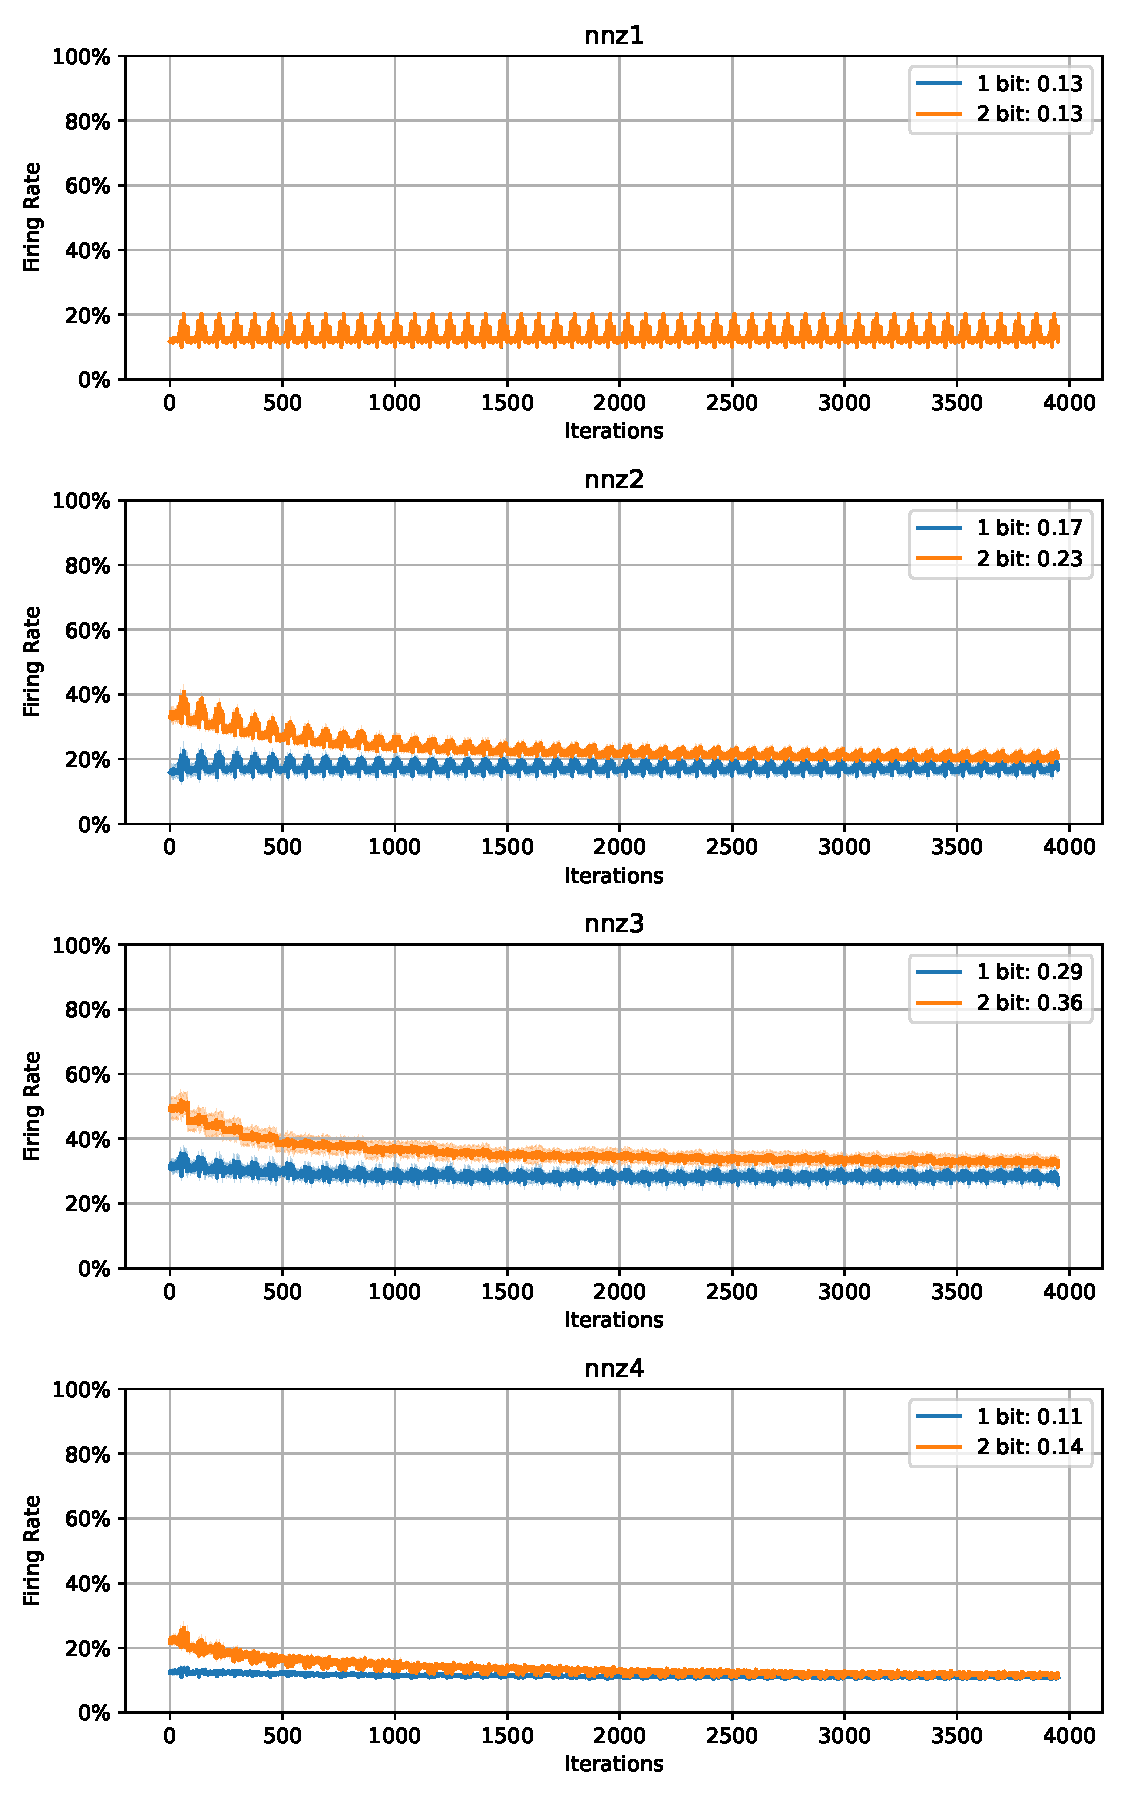
\includegraphics[width=\textwidth]{../firerate/MNIST/plots/mnist_test_firerate.pdf}
                \caption{Firing Rate in Different Positions (Test)}
            \end{subfigure}
        \end{figure}
        \begin{figure}[H]
            \centering
            \ContinuedFloat
            \begin{subfigure}[H]{\textwidth}
                \centering
                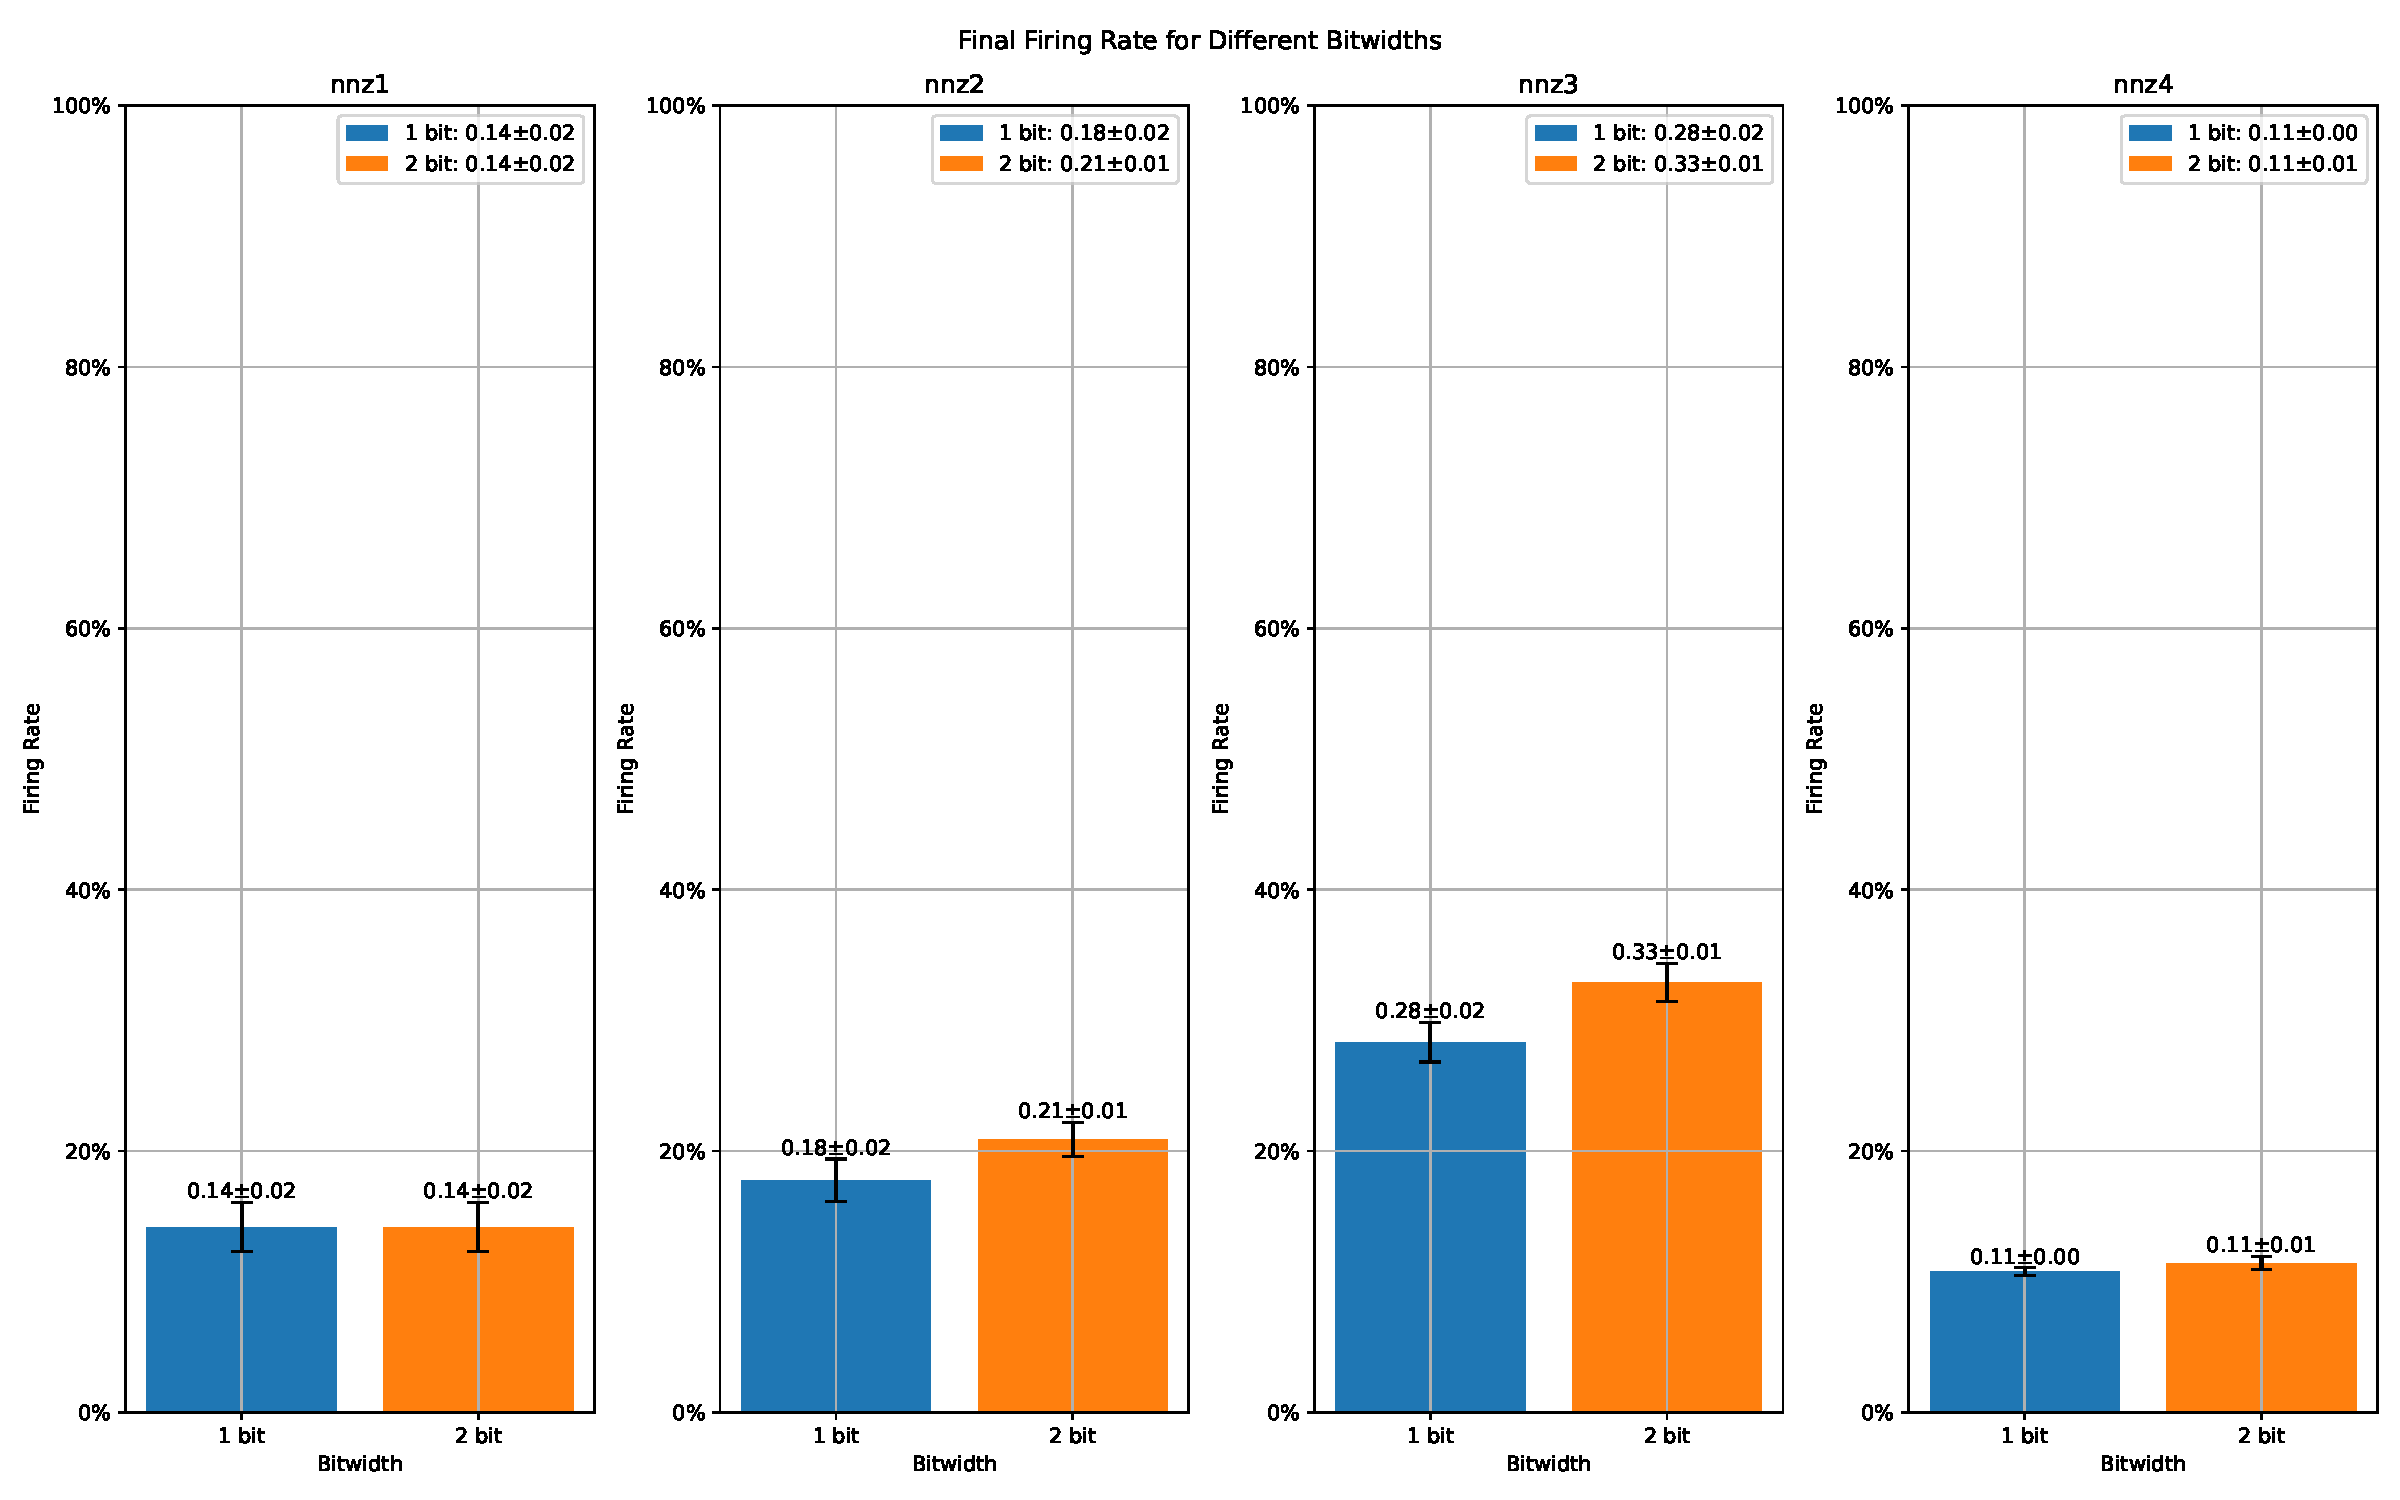
\includegraphics[width=\textwidth]{../firerate/MNIST/plots/mnist_final_firerate.pdf}
                \caption{Firing Rate in Different Positions (Final Test)}
            \end{subfigure}
            \caption{Firing Rate in Different Positions of the MNIST Model}
        \end{figure}

    \section{NMNIST}
    \label{appendix:firerate_nmnist}
        \begin{figure}[H]
            \centering
            \begin{subfigure}[H]{0.8\textwidth}
                \centering
                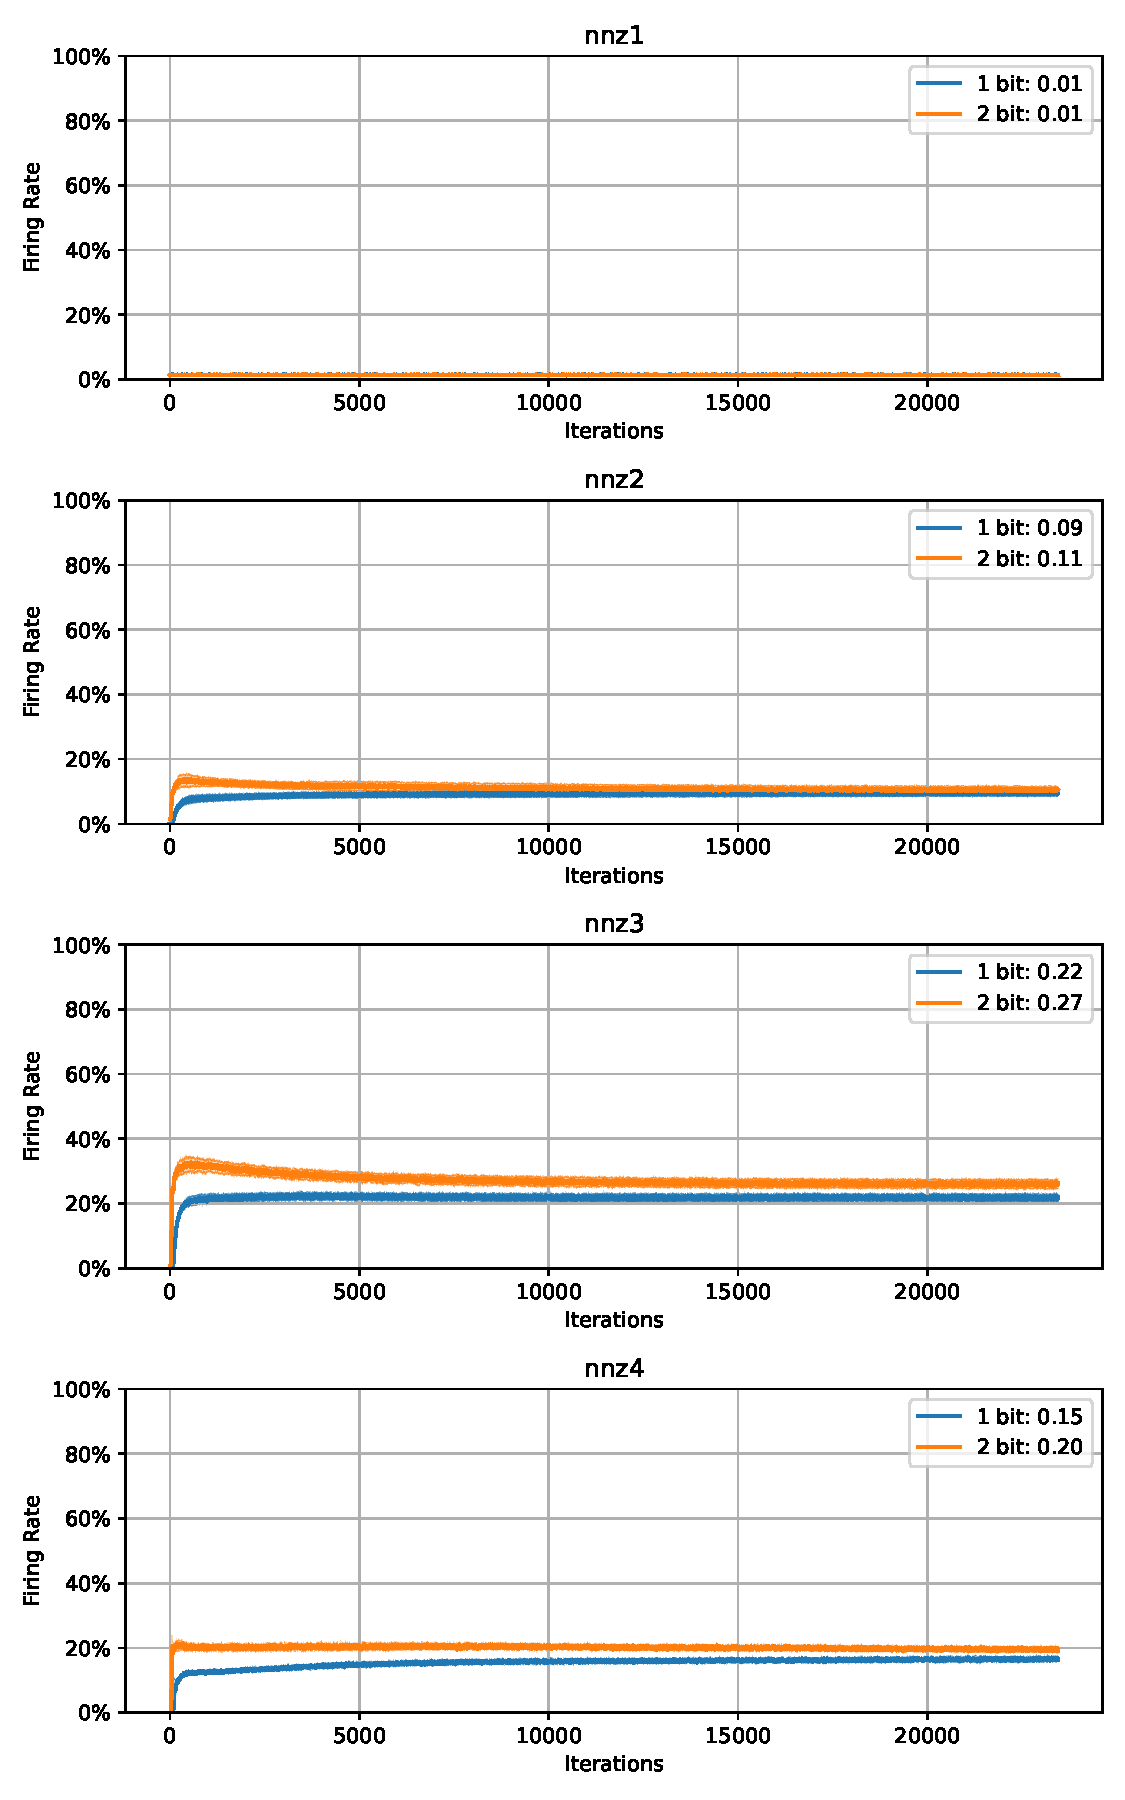
\includegraphics[width=\textwidth]{../firerate/NMNIST/plots/nmnist_train_firerate.pdf}
                \caption{Firing Rate in Different Positions (Training)}
            \end{subfigure}
        \end{figure}
        \begin{figure}[H]
            \centering
            \ContinuedFloat
            \begin{subfigure}[H]{0.8\textwidth}
                \centering
                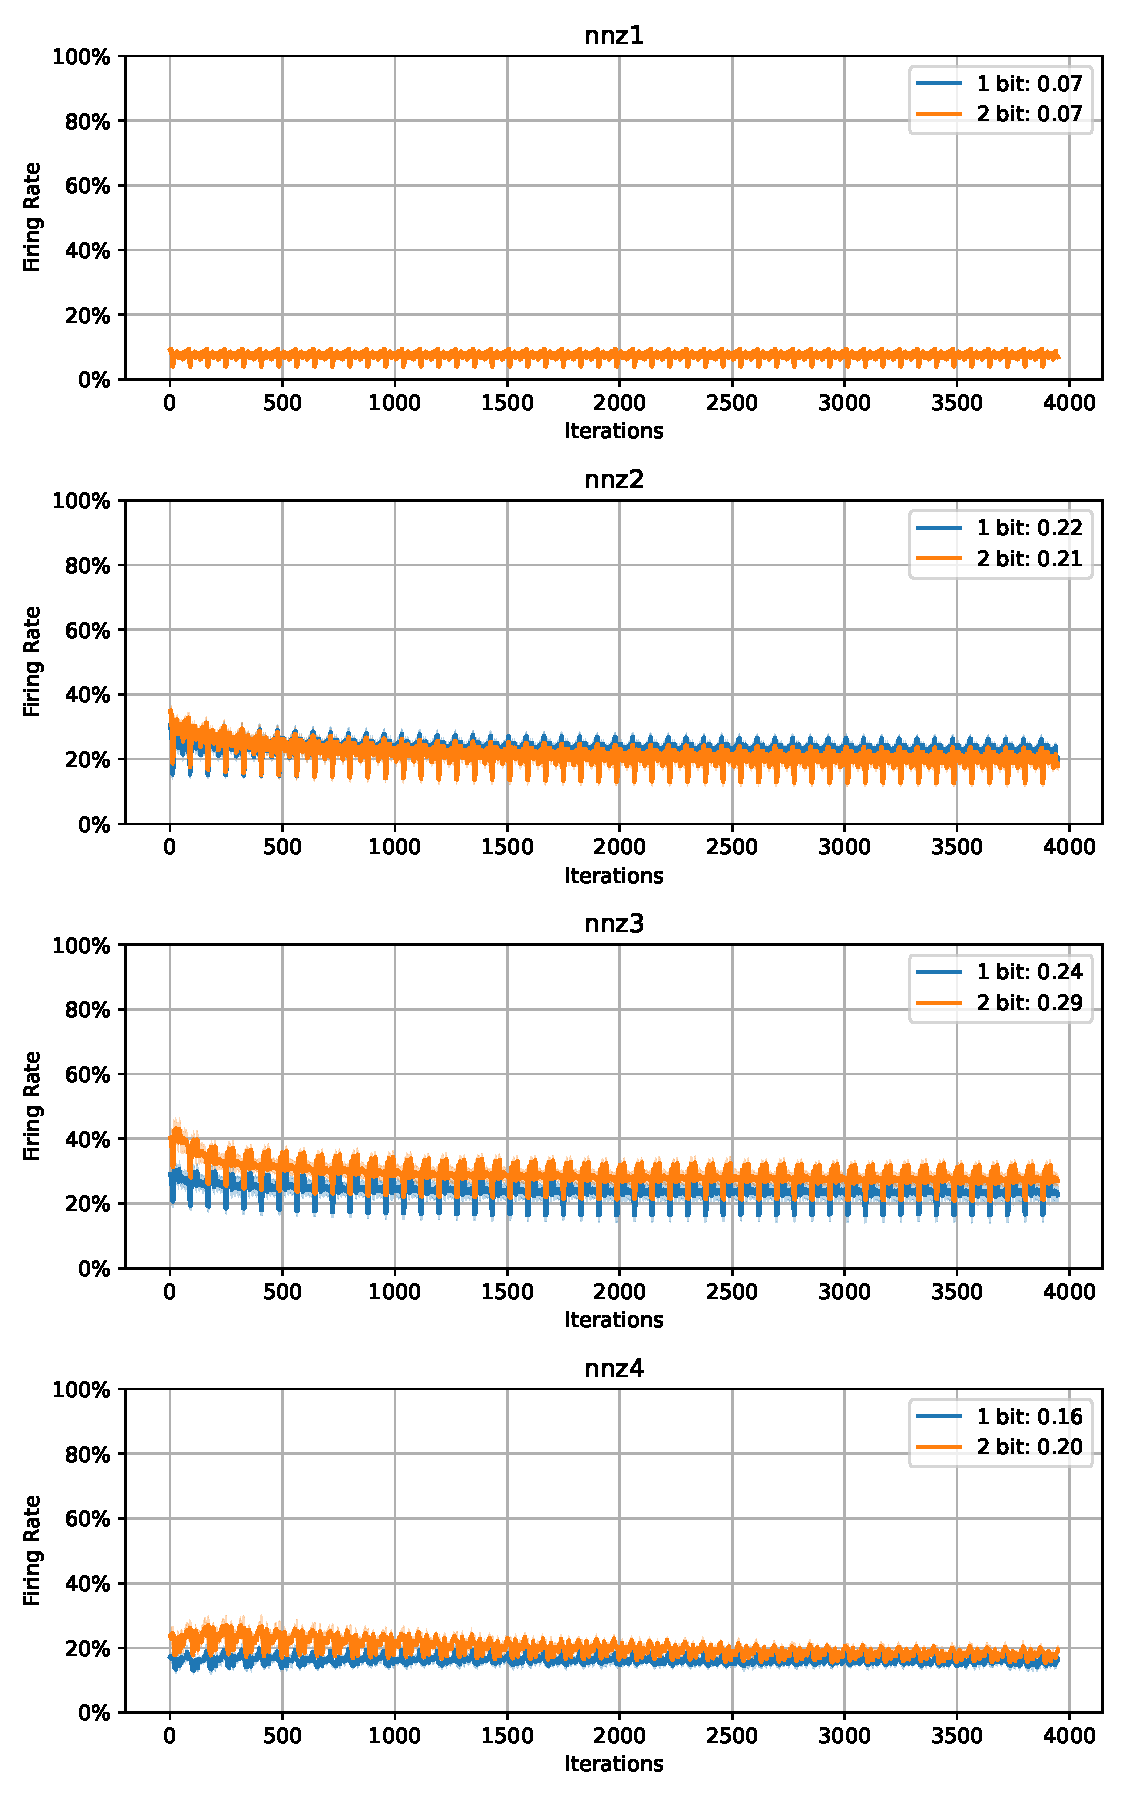
\includegraphics[width=\textwidth]{../firerate/NMNIST/plots/nmnist_test_firerate.pdf}
                \caption{Firing Rate in Different Positions (Test)}
            \end{subfigure}
        \end{figure}
        \begin{figure}[H]
            \centering
            \ContinuedFloat
            \begin{subfigure}[H]{\textwidth}
                \centering
                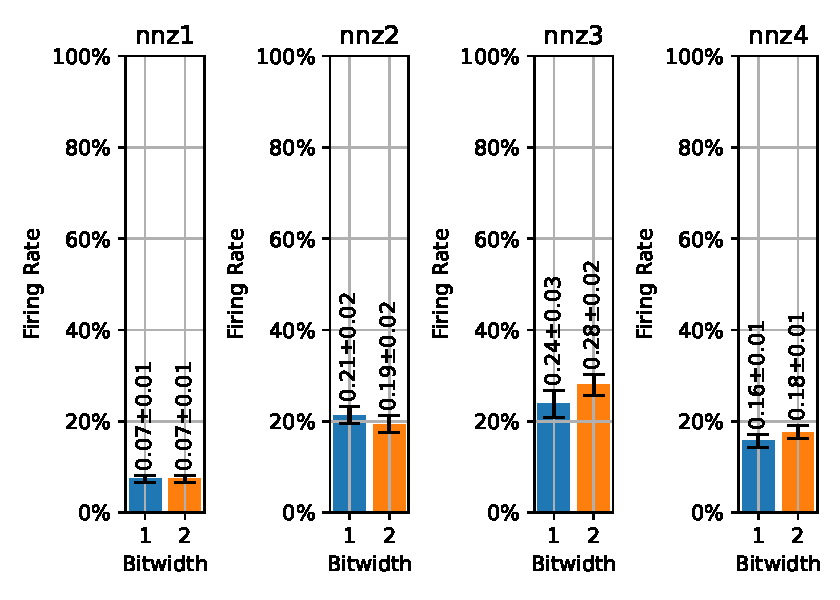
\includegraphics[width=\textwidth]{../firerate/NMNIST/plots/nmnist_final_firerate.pdf}
                \caption{Firing Rate in Different Positions (Final Test)}
            \end{subfigure}
            \caption{Firing Rate in Different Positions of the NMNIST Model}
        \end{figure}

    \section{DVS Gesture}
    \label{appendix:firerate_dvs_gesture}
        \begin{figure}[H]
            \centering
            \begin{subfigure}[H]{0.8\textwidth}
                \centering
                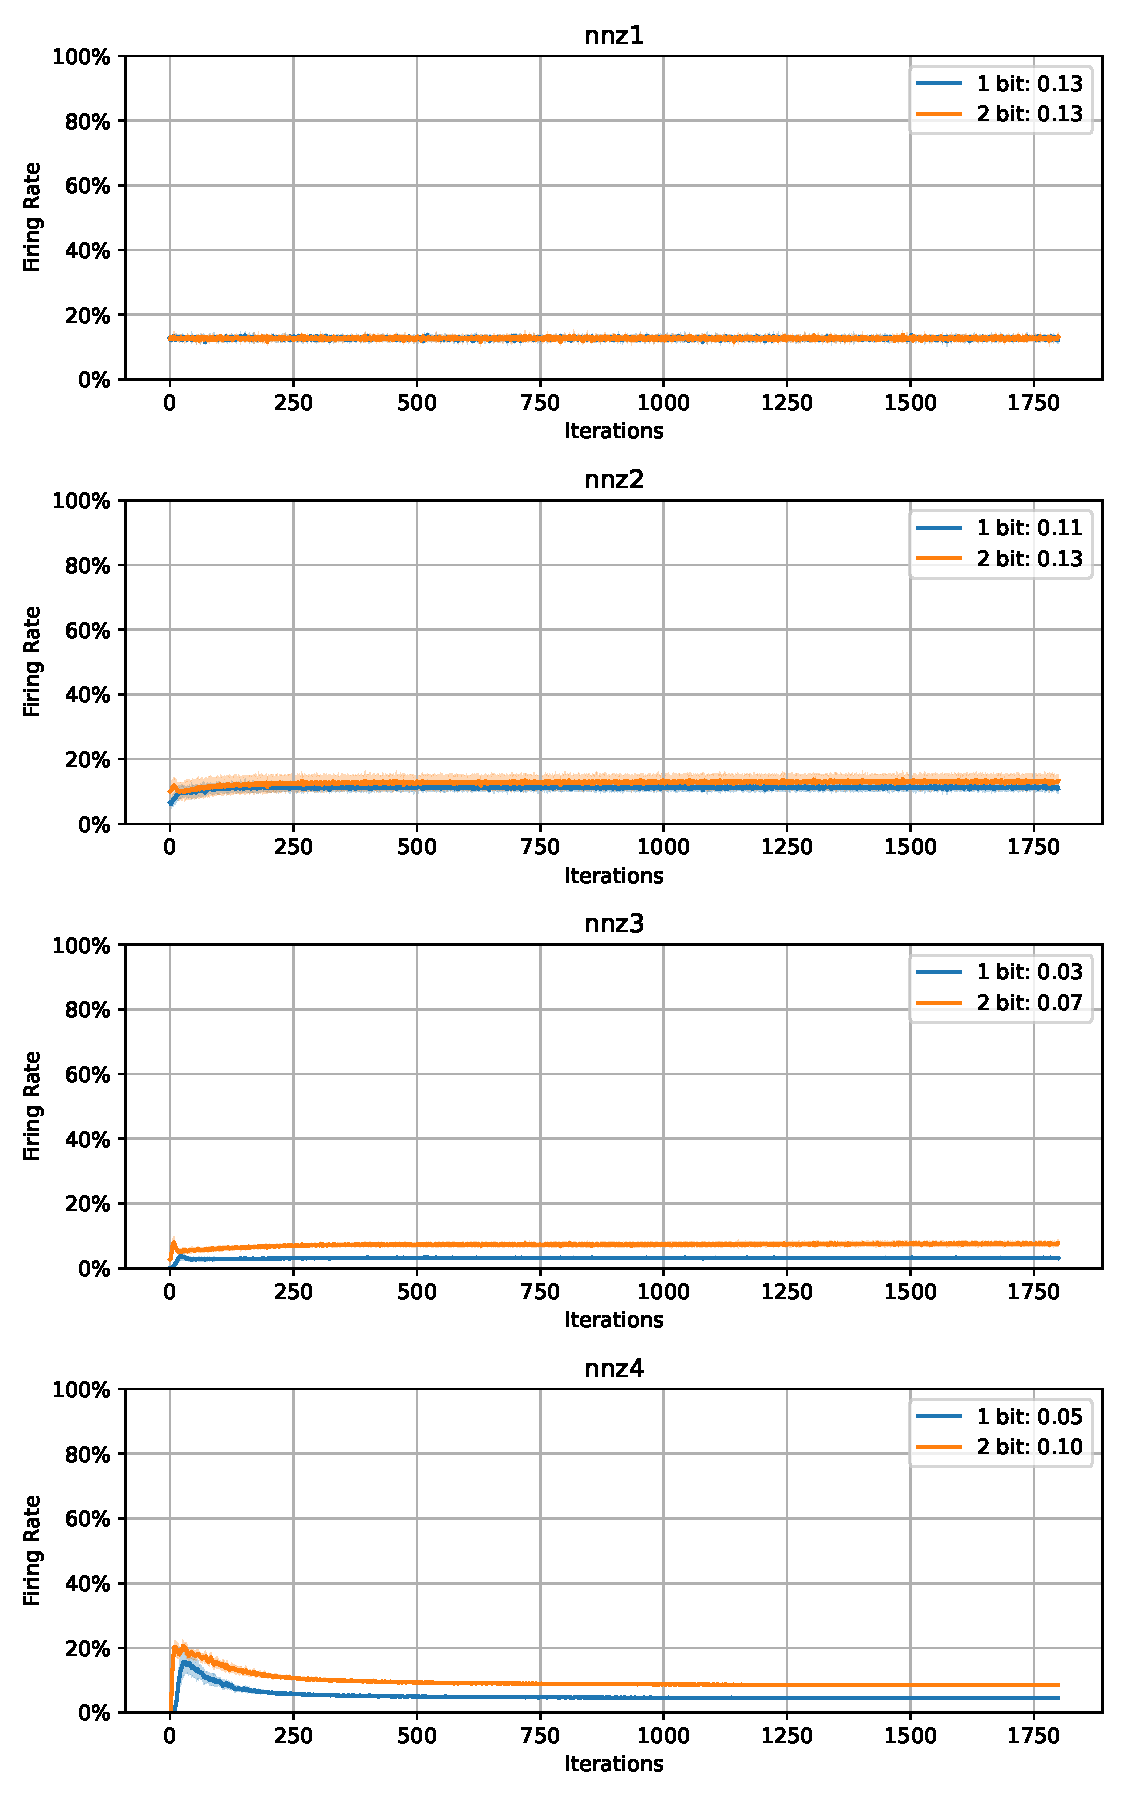
\includegraphics[width=\textwidth]{../firerate/DVSGesture/plots/dvsgesture_train_firerate.pdf}
                \caption{Firing Rate in Different Positions (Training)}
            \end{subfigure}
        \end{figure}
        \begin{figure}[H]
            \centering
            \ContinuedFloat
            \begin{subfigure}[H]{0.8\textwidth}
                \centering
                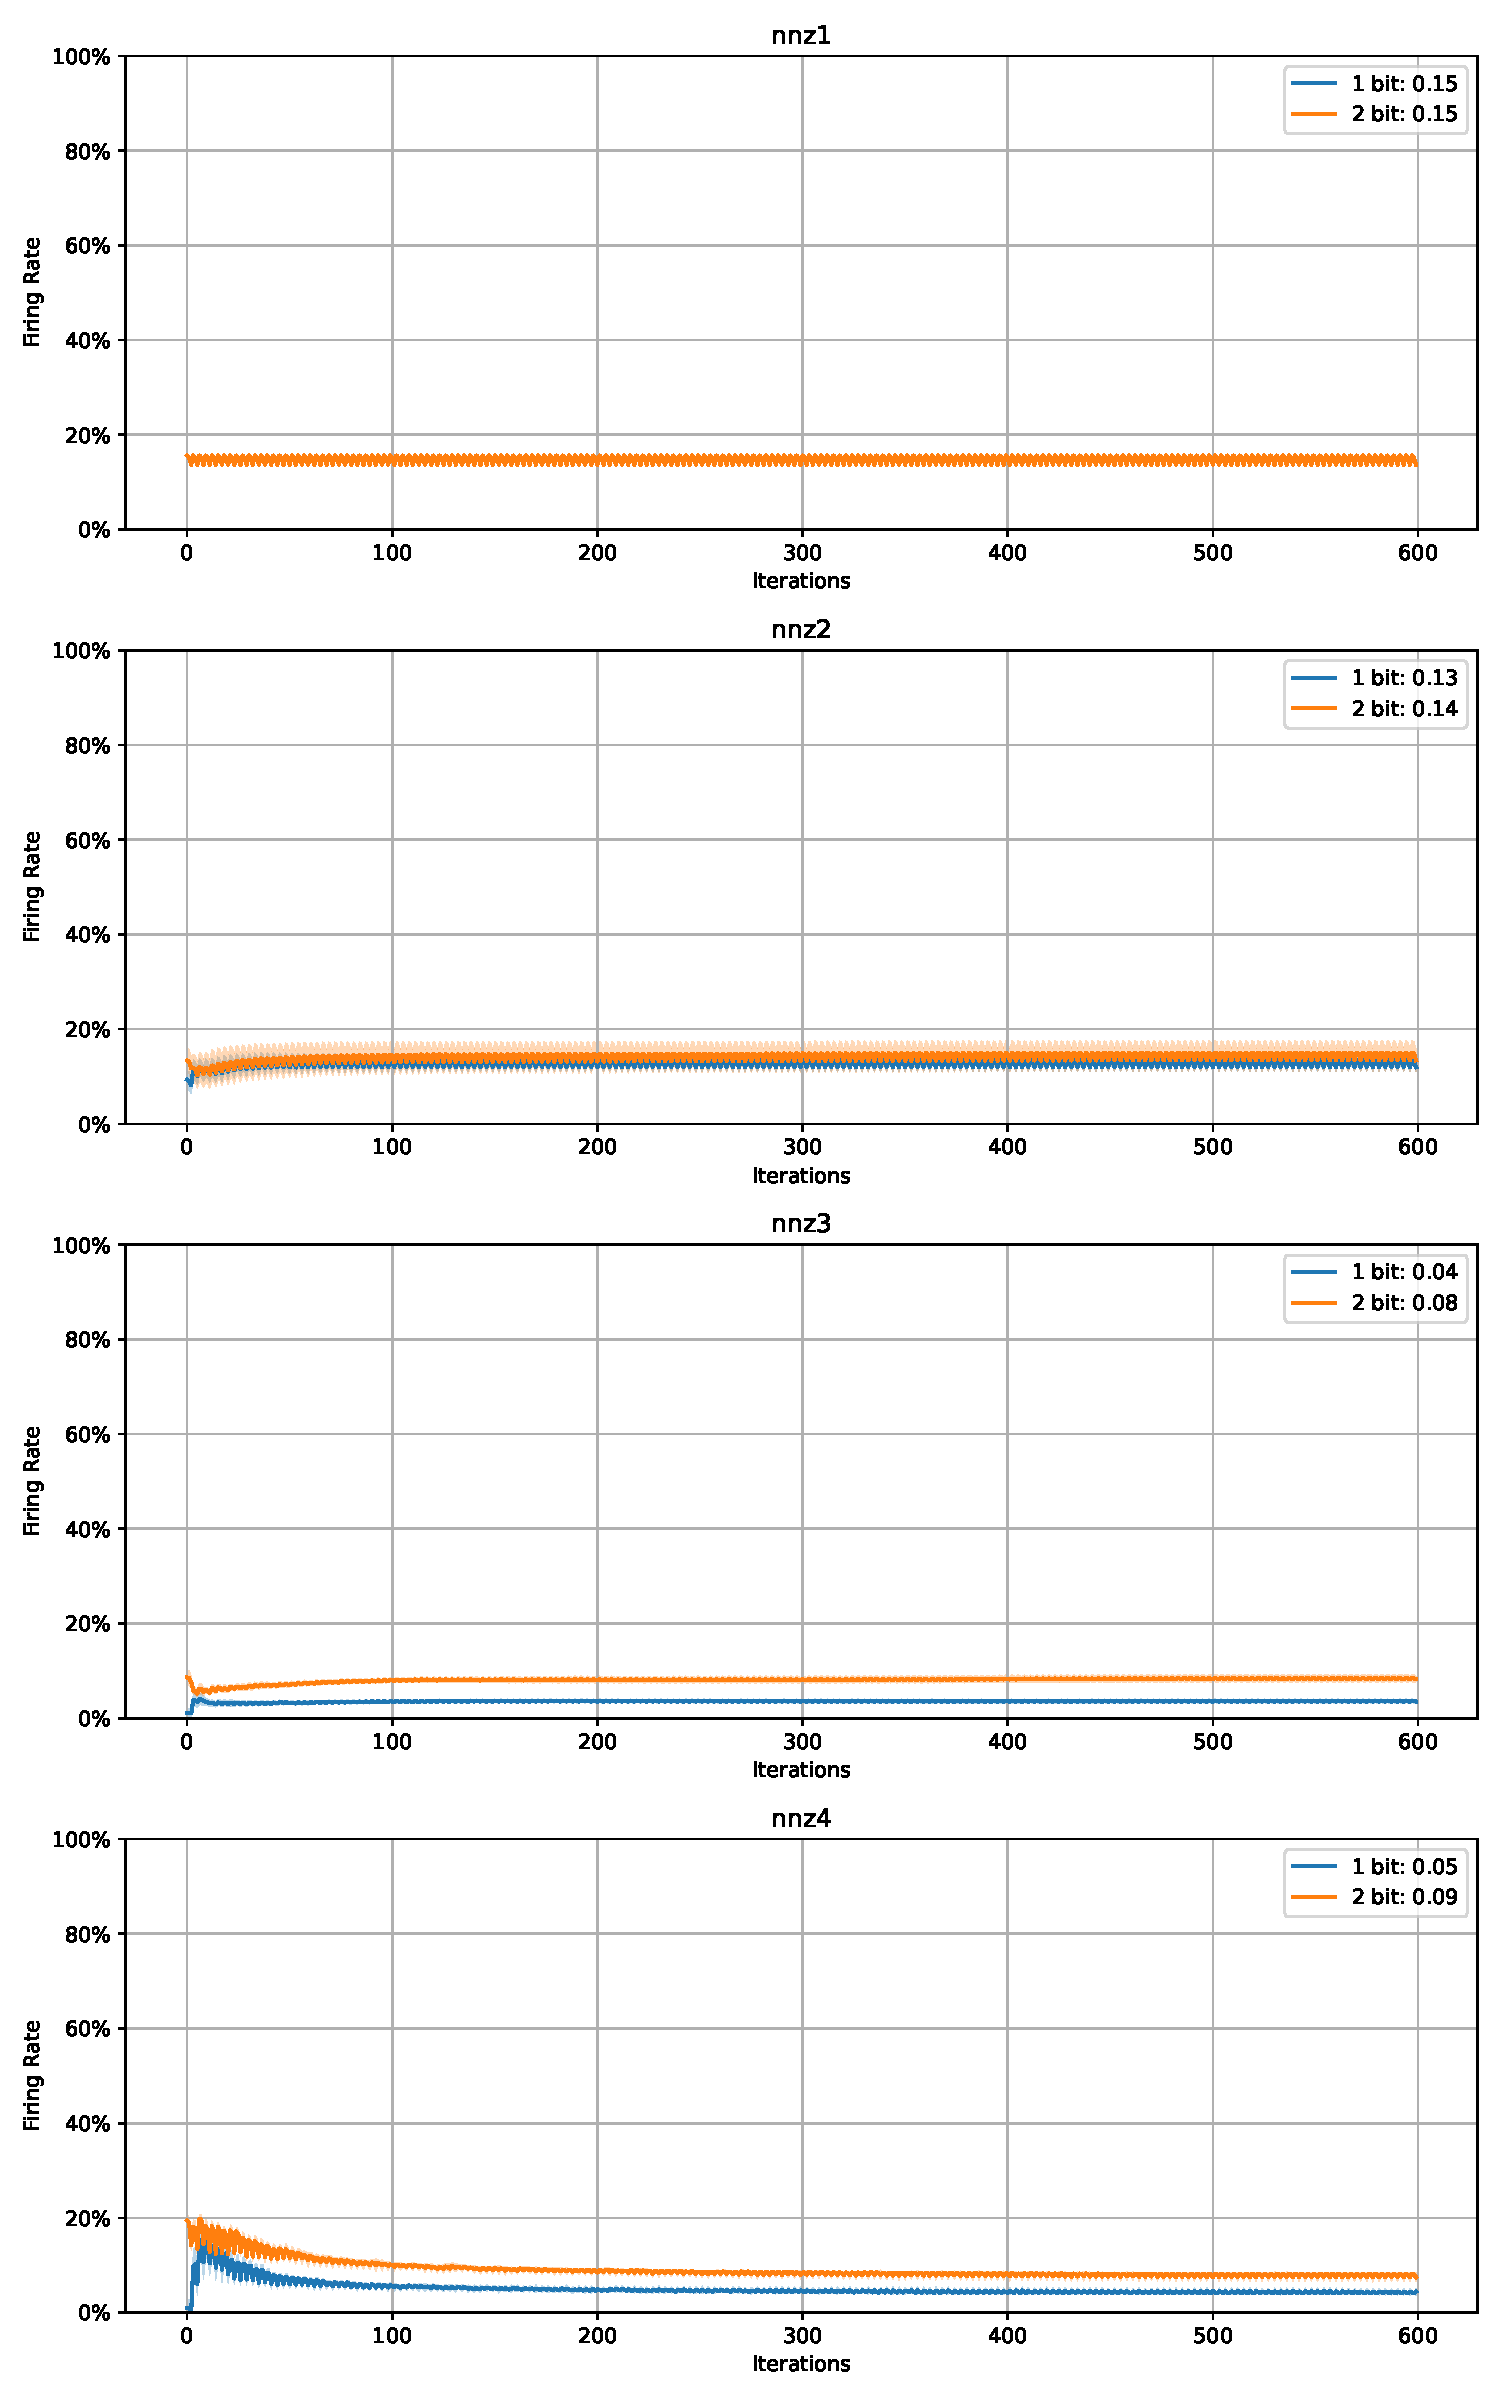
\includegraphics[width=\textwidth]{../firerate/DVSGesture/plots/dvsgesture_test_firerate.pdf}
                \caption{Firing Rate in Different Positions (Test)}
            \end{subfigure}
        \end{figure}
        \begin{figure}[H]
            \centering
            \ContinuedFloat
            \begin{subfigure}[H]{\textwidth}
                \centering
                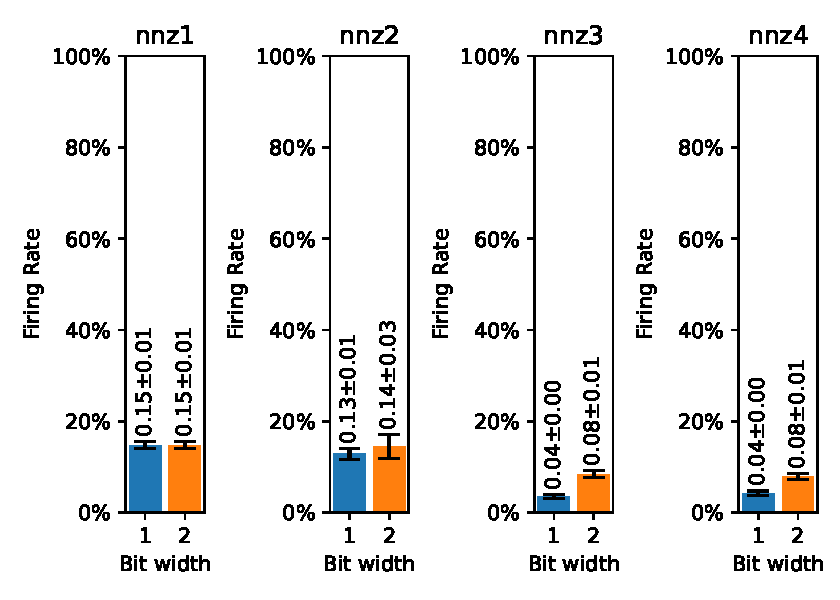
\includegraphics[width=\textwidth]{../firerate/DVSGesture/plots/dvsgesture_final_firerate.pdf}
                \caption{Firing Rate in Different Positions (Final Test)}
            \end{subfigure}
            \caption{Firing Rate in Different Positions of the DVS Gesture Model}
        \end{figure}

    \section{CIFAR-10}
    \label{appendix:firerate_cifar10}
        Here we use learning rate schedulers to accelerate the convergence of the models. Although the models can reach a high accuracy faster, the multi-bit spike train model suffers from the high learning rate from time to time. 

        \begin{figure}[H]
            \centering
            \begin{subfigure}[H]{0.8\textwidth}
                \centering
                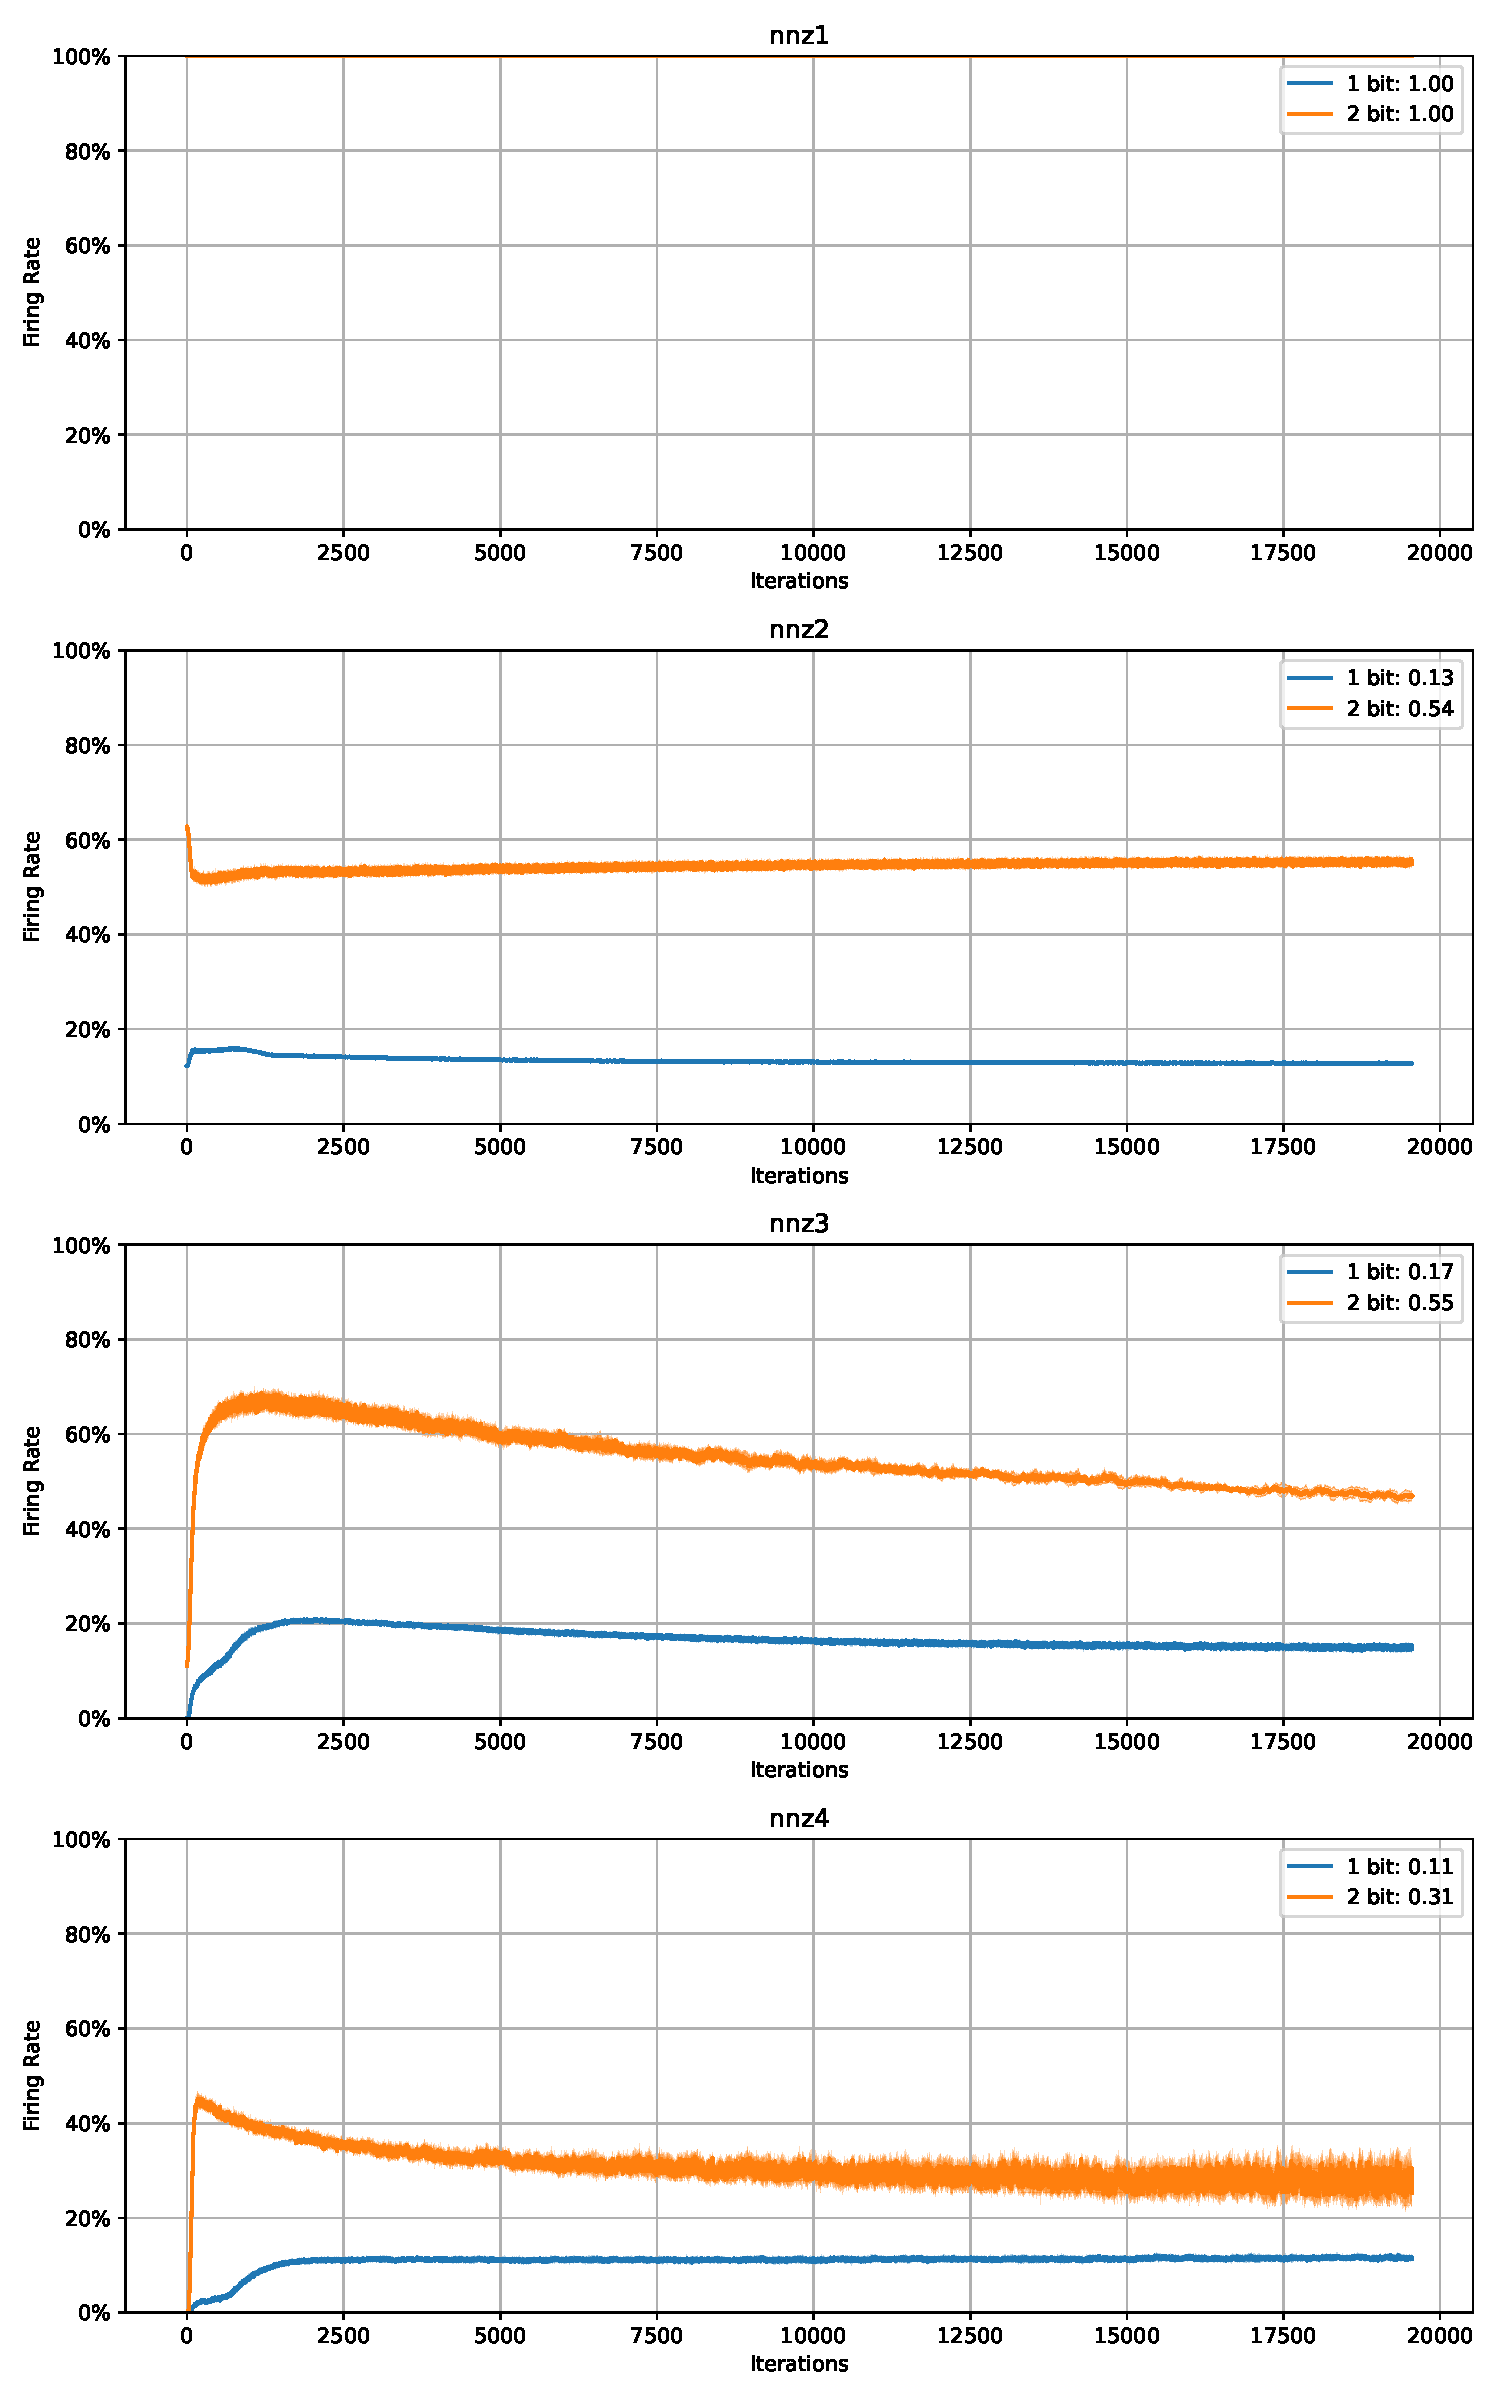
\includegraphics[width=\textwidth]{../firerate/CIFAR10/plots/cifar10_train_firerate.pdf}
                \caption{Firing Rate in Different Positions (Training)}
            \end{subfigure}
        \end{figure}
        \begin{figure}[H]
            \centering
            \ContinuedFloat
            \begin{subfigure}[H]{0.8\textwidth}
                \centering
                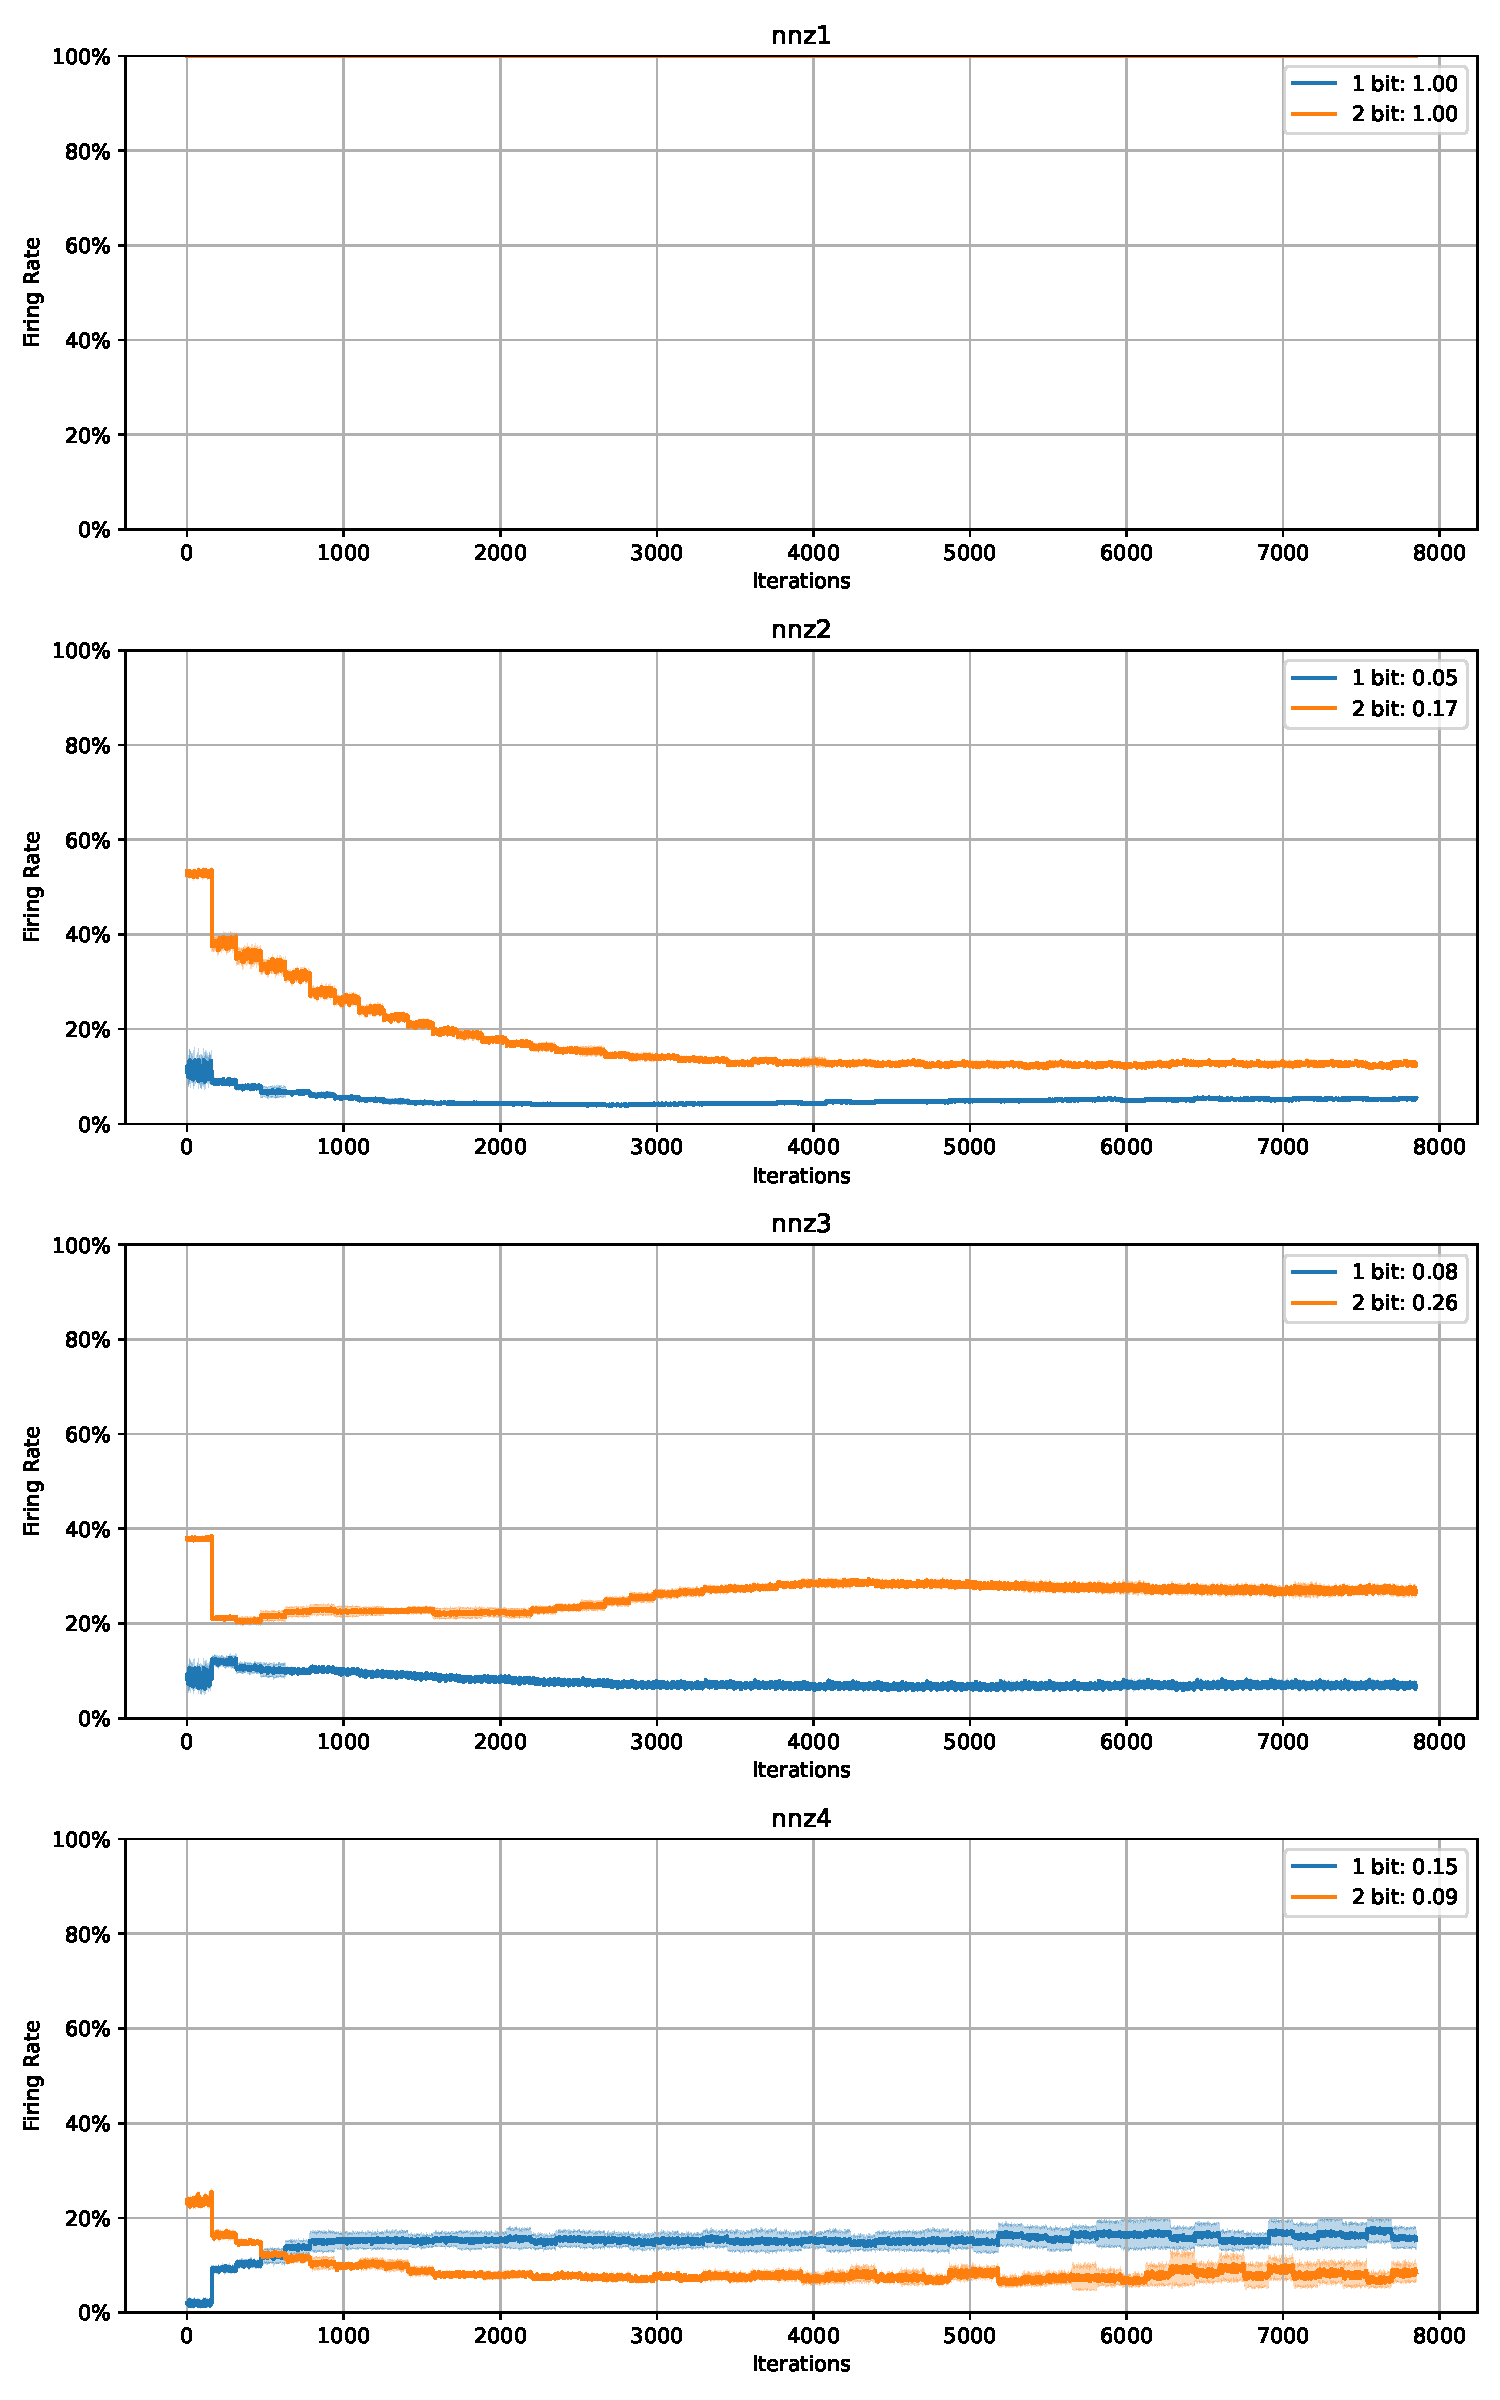
\includegraphics[width=\textwidth]{../firerate/CIFAR10/plots/cifar10_test_firerate.pdf}
                \caption{Firing Rate in Different Positions (Test)}
            \end{subfigure}
        \end{figure}
        \begin{figure}[H]
            \centering
            \ContinuedFloat
            \begin{subfigure}[H]{\textwidth}
                \centering
                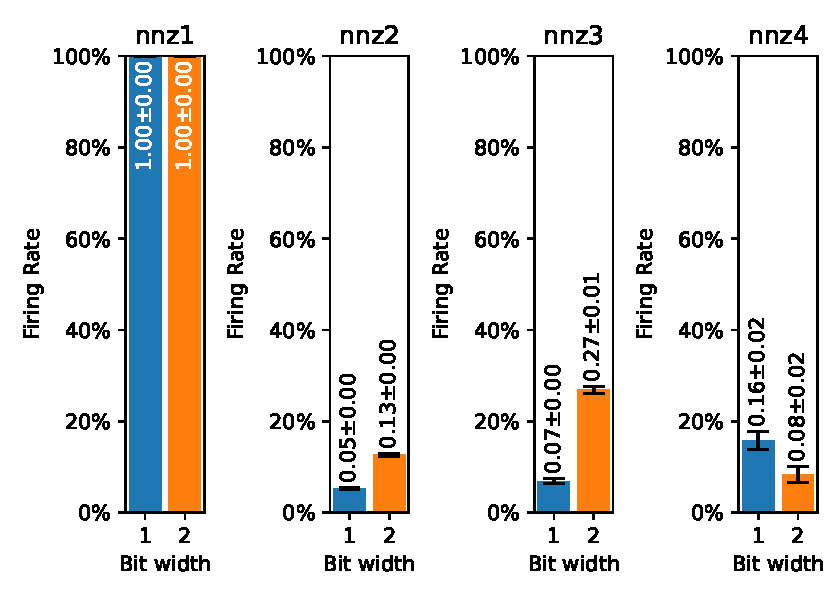
\includegraphics[width=\textwidth]{../firerate/CIFAR10/plots/cifar10_final_firerate.pdf}
                \caption{Firing Rate in Different Positions (Final Test)}
            \end{subfigure}
            \caption{Firing Rate in Different Positions of the CIFAR-10 Model}
        \end{figure}

\chapter{Energy Consumption Estimation}
\label{appendix:energy}

\section{Training Energy Consumption Estimation on GPUs}
\label{appendix:energy_gpu}

    The hyperparameters used in the training process are the same as in Table \ref{tab:hyperparameters_accuracy}.

    \label{appendix:energy_gpu_fashion_mnist}

        \begin{figure}[H]
            \centering
            \begin{subfigure}[H]{0.6\textwidth}
                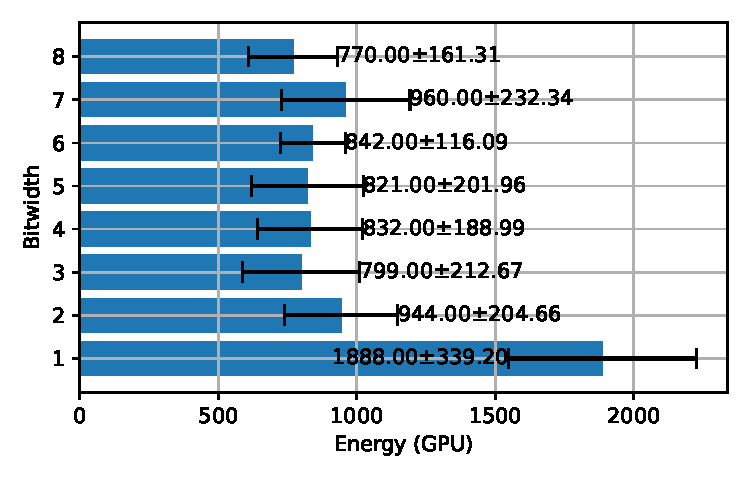
\includegraphics[width=\textwidth]{../standard/FashionMNIST/plots/fashionmnist_train_energy_gpu_horizontal.pdf}
                \caption{Energy Consumption Estimation, Unit in Constant $c$}
            \end{subfigure}
        \end{figure}
        \begin{figure}[H]
            \centering
            \ContinuedFloat
            \begin{subfigure}[H]{0.6\textwidth}
                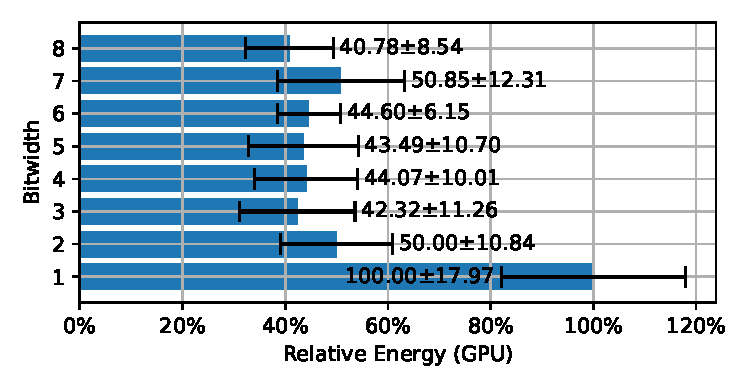
\includegraphics[width=\textwidth]{../standard/FashionMNIST/plots/fashionmnist_train_relative_energy_gpu_horizontal.pdf}
                \caption{Normalized Energy Consumption Estimation Relative to 1-bit Spike Train Model}
            \end{subfigure}
            \caption{Training Energy Consumption Estimation on GPUs for Fashion MNIST Dataset}
        \end{figure}

    \label{appendix:energy_gpu_mnist}

        \begin{figure}[H]
            \centering
            \begin{subfigure}[H]{0.6\textwidth}
                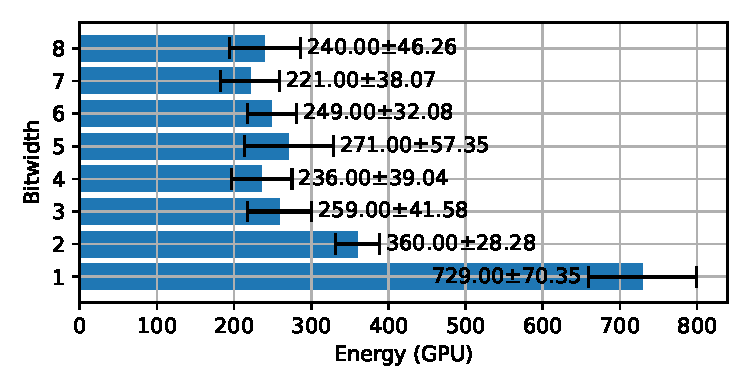
\includegraphics[width=\textwidth]{../standard/MNIST/plots/mnist_train_energy_gpu_horizontal.pdf}
                \caption{Energy Consumption Estimation, Unit in Constant $c$}
            \end{subfigure}
        \end{figure}
        \begin{figure}[H]
            \centering
            \ContinuedFloat
            \begin{subfigure}[H]{0.6\textwidth}
                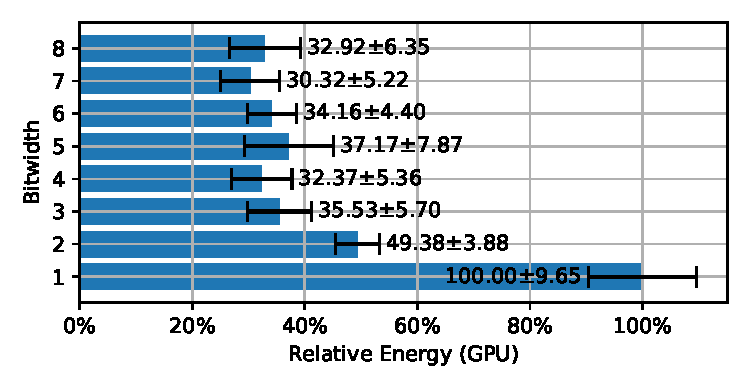
\includegraphics[width=\textwidth]{../standard/MNIST/plots/mnist_train_relative_energy_gpu_horizontal.pdf}
                \caption{Normalized Energy Consumption Estimation Relative to 1-bit Spike Train Model}
            \end{subfigure}
            \caption{Training Energy Consumption Estimation on GPUs for MNIST Dataset}
        \end{figure}

    \label{appendix:energy_gpu_nmnist}

        \begin{figure}[H]
            \centering
            \begin{subfigure}[H]{0.6\textwidth}
                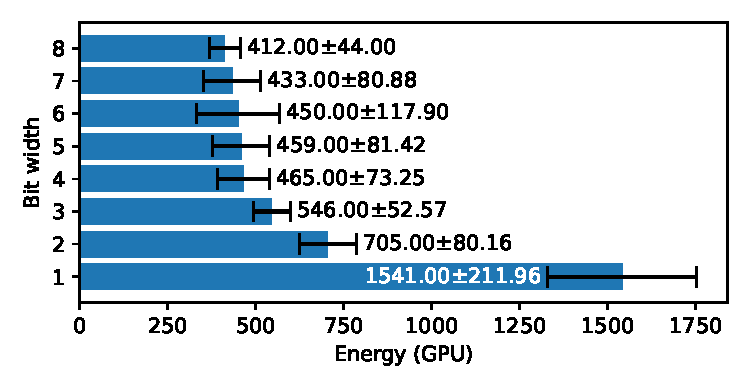
\includegraphics[width=\textwidth]{../standard/NMNIST/plots/nmnist_train_energy_gpu_horizontal.pdf}
                \caption{Energy Consumption Estimation, Unit in Constant $c$}
            \end{subfigure}
        \end{figure}
        \begin{figure}[H]
            \centering
            \ContinuedFloat
            \begin{subfigure}[H]{0.6\textwidth}
                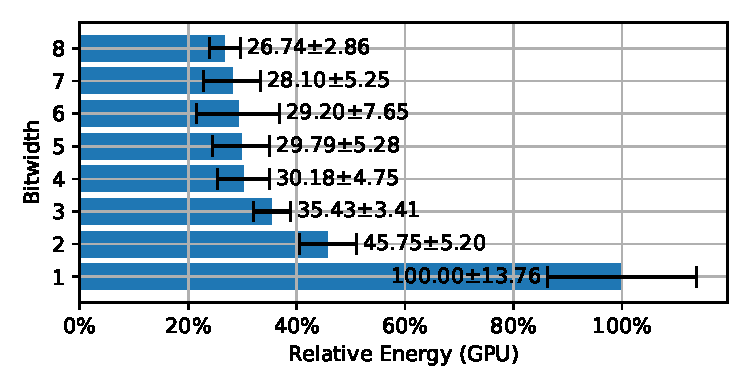
\includegraphics[width=\textwidth]{../standard/NMNIST/plots/nmnist_train_relative_energy_gpu_horizontal.pdf}
                \caption{Normalized Energy Consumption Estimation Relative to 1-bit Spike Train Model}
            \end{subfigure}
            \caption{Training Energy Consumption Estimation on GPUs for NMNIST Dataset}
        \end{figure}

    \label{appendix:energy_gpu_dvs_gesture}

        \begin{figure}[H]
            \centering
            \begin{subfigure}[H]{0.6\textwidth}
                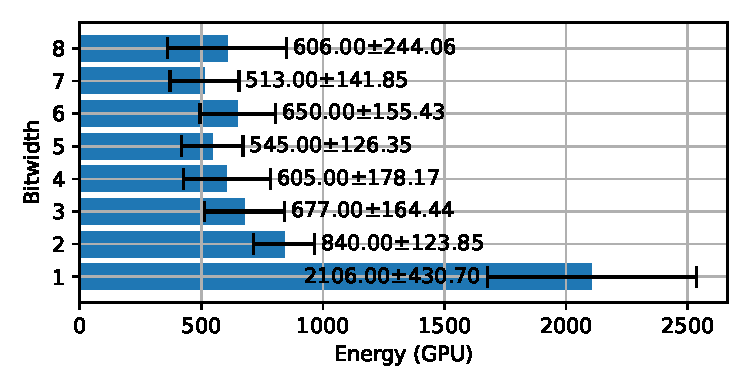
\includegraphics[width=\textwidth]{../standard/DVSGesture/plots/dvsgesture_train_energy_gpu_horizontal.pdf}
                \caption{Energy Consumption Estimation, Unit in Constant $c$}
            \end{subfigure}
        \end{figure}
        \begin{figure}[H]
            \centering
            \ContinuedFloat
            \begin{subfigure}[H]{0.6\textwidth}
                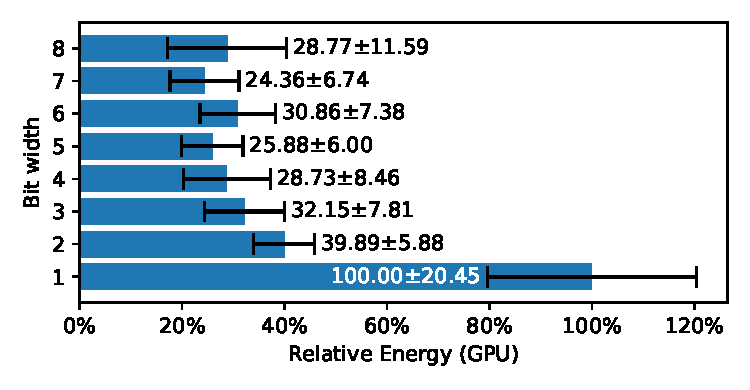
\includegraphics[width=\textwidth]{../standard/DVSGesture/plots/dvsgesture_train_relative_energy_gpu_horizontal.pdf}
                \caption{Normalized Energy Consumption Estimation Relative to 1-bit Spike Train Model}
            \end{subfigure}
            \caption{Training Energy Consumption Estimation on GPUs for DVS Gesture Dataset}
        \end{figure}

    \label{appendix:energy_gpu_cifar10}

        \begin{figure}[H]
            \centering
            \begin{subfigure}[H]{0.6\textwidth}
                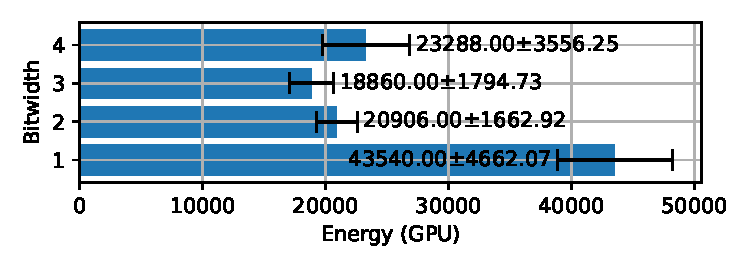
\includegraphics[width=\textwidth]{../standard/CIFAR10/plots/cifar10_train_energy_gpu_horizontal.pdf}
                \caption{Energy Consumption Estimation, Unit in Constant $c$}
            \end{subfigure}
        \end{figure}
        \begin{figure}[H]
            \centering
            \ContinuedFloat
            \begin{subfigure}[H]{0.6\textwidth}
                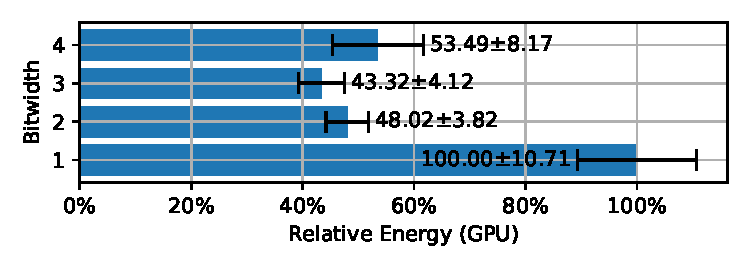
\includegraphics[width=\textwidth]{../standard/CIFAR10/plots/cifar10_train_relative_energy_gpu_horizontal.pdf}
                \caption{Normalized Energy Consumption Estimation Relative to 1-bit Spike Train Model}
            \end{subfigure}
            \caption{Training Energy Consumption Estimation on GPUs for CIFAR-10 Dataset}
        \end{figure}

\section{Inference Energy Consumption Estimation on Neuromorphic Hardware}
\label{appendix:energy_neuromorphic}

    We assume the models are running on neuromorphic hardware like Intel Loihi 2 that support graded spikes. 

    The hyperparameters used in the training process are the same as in Table \ref{tab:hyperparameters_accuracy}.

    \subsection{Fashion MNIST}
    \label{appendix:energy_neuromorphic_fashion_mnist}

        \begin{figure}[H]
            \centering
            \begin{subfigure}[H]{0.495\textwidth}
                \includegraphics[width=\textwidth]{../standard/FashionMNIST/plots/fashionmnist_test_energy_nh.pdf}
                \caption{Energy Consumption Estimation, Unit in Parameters $F\cdot E_{\text{MAC}}$}
            \end{subfigure}
            \hfill
            \begin{subfigure}[H]{0.495\textwidth}
                \includegraphics[width=\textwidth]{../standard/FashionMNIST/plots/fashionmnist_test_relative_energy_nh.pdf}
                \caption{Normalized Energy Consumption Estimation Relative to 1-bit Spike Train Model}
            \end{subfigure}
            \caption{Inference Energy Consumption Estimation on Intel Loihi 2}
        \end{figure}
    
    \subsection{MNIST}
    \label{appendix:energy_neuromorphic_mnist}

        \begin{figure}[H]
            \centering
            \begin{subfigure}[H]{0.495\textwidth}
                \includegraphics[width=\textwidth]{../standard/MNIST/plots/mnist_test_energy_nh.pdf}
                \caption{Energy Consumption Estimation, Unit in Parameters $F\cdot E_{\text{MAC}}$}
            \end{subfigure}
            \hfill
            \begin{subfigure}[H]{0.495\textwidth}
                \includegraphics[width=\textwidth]{../standard/MNIST/plots/mnist_test_relative_energy_nh.pdf}
                \caption{Normalized Energy Consumption Estimation Relative to 1-bit Spike Train Model}
            \end{subfigure}
            \caption{Inference Energy Consumption Estimation on Intel Loihi 2}
        \end{figure}

    \subsection{NMNIST}
    \label{appendix:energy_neuromorphic_nmnist}

        \begin{figure}[H]
            \centering
            \begin{subfigure}[H]{0.495\textwidth}
                \includegraphics[width=\textwidth]{../standard/NMNIST/plots/nmnist_test_energy_nh.pdf}
                \caption{Energy Consumption Estimation, Unit in Parameters $F\cdot E_{\text{MAC}}$}
            \end{subfigure}
            \hfill
            \begin{subfigure}[H]{0.495\textwidth}
                \includegraphics[width=\textwidth]{../standard/NMNIST/plots/nmnist_test_relative_energy_nh.pdf}
                \caption{Normalized Energy Consumption Estimation Relative to 1-bit Spike Train Model}
            \end{subfigure}
            \caption{Inference Energy Consumption Estimation on Intel Loihi 2}
        \end{figure}

    \subsection{DVS Gesture}
    \label{appendix:energy_neuromorphic_dvs_gesture}

        \begin{figure}[H]
            \centering
            \begin{subfigure}[H]{0.495\textwidth}
                \includegraphics[width=\textwidth]{../standard/DVSGesture/plots/dvsgesture_test_energy_nh.pdf}
                \caption{Energy Consumption Estimation, Unit in Parameters $F\cdot E_{\text{MAC}}$}
            \end{subfigure}
            \hfill
            \begin{subfigure}[H]{0.495\textwidth}
                \includegraphics[width=\textwidth]{../standard/DVSGesture/plots/dvsgesture_test_relative_energy_nh.pdf}
                \caption{Normalized Energy Consumption Estimation Relative to 1-bit Spike Train Model}
            \end{subfigure}
            \caption{Inference Energy Consumption Estimation on Intel Loihi 2}
        \end{figure}

    \subsection{CIFAR-10}
    \label{appendix:energy_neuromorphic_cifar10}

        \begin{figure}[H]
            \centering
            \begin{subfigure}[H]{0.495\textwidth}
                \includegraphics[width=\textwidth]{../standard/CIFAR10/plots/cifar10_test_energy_nh.pdf}
                \caption{Energy Consumption Estimation, Unit in Parameters $F\cdot E_{\text{MAC}}$}
            \end{subfigure}
            \hfill
            \begin{subfigure}[H]{0.495\textwidth}
                \includegraphics[width=\textwidth]{../standard/CIFAR10/plots/cifar10_test_relative_energy_nh.pdf}
                \caption{Normalized Energy Consumption Estimation Relative to 1-bit Spike Train Model}
            \end{subfigure}
            \caption{Inference Energy Consumption Estimation on Intel Loihi 2}
        \end{figure}

\section{Trading Accuracy for Energy Consumption}
\label{appendix:energy_tradeoff}

    The hyperparameters used in the training process are shown in Table \ref{tab:hyperparameters_energy_tradeoff}.

    \begin{table}[H]
        \begin{tabularx}{\textwidth}{|X|c|c|c|c|c|c|c|}
            \toprule
            Dataset & Reps & Epochs & LR & Opt & Batch & Time steps \\
            \midrule
            Fashion MNIST & 10 & 5 & 2e-3 & Adam & 128 & 4 \\
            CIFAR-10 & 5 & 50 & 1e-5 & Adam & 128 & 4 \\
            \bottomrule
        \end{tabularx}
        \caption{Hyperparameters}
        \label{tab:hyperparameters_energy_tradeoff}
    \end{table}

    \subsection{Fashion MNIST}
    \label{appendix:energy_tradeoff_fashion_mnist}

        \begin{figure}[H]
            \centering
            \begin{subfigure}[H]{0.89\textwidth}
                \centering
                \begin{subfigure}[H]{\textwidth}
                    \includegraphics[width=\textwidth]{../timesteps/FashionMNIST/plots/fashionmnist_train_acc.pdf}
                    \caption{Training Accuracy (smoothed with a window size of 100)}
                \end{subfigure}
                \hfill
                \begin{subfigure}[H]{\textwidth}
                    \includegraphics[width=\textwidth]{../timesteps/FashionMNIST/plots/fashionmnist_test_acc.pdf}
                    \caption{Test Accuracy}
                \end{subfigure}
            \end{subfigure}
            \hfill
            \begin{subfigure}[H]{0.1\textwidth}
                \includegraphics[width=\textwidth]{../timesteps/FashionMNIST/plots/fashionmnist_final_acc.pdf}
                \caption{Final Test Accuracy}
            \end{subfigure}
            \caption{Accuracy of 1-bit Spike Train Model with 10 Timesteps and 2-bit Spike Train Model with 4 Timesteps}
        \end{figure}

        \begin{figure}[H]
            \centering
            \begin{subfigure}[H]{\textwidth}
                \includegraphics[width=\textwidth]{../timesteps/FashionMNIST/plots/fashionmnist_train_energy_gpu_horizontal.pdf}
                \caption{Energy Consumption Estimation, Unit in Constant $c$}
            \end{subfigure}
            \hfill
            \begin{subfigure}[H]{\textwidth}
                \includegraphics[width=\textwidth]{../timesteps/FashionMNIST/plots/fashionmnist_train_relative_energy_gpu_horizontal.pdf}
                \caption{Normalized Energy Consumption Estimation Relative to 1-bit Spike Train Model}
            \end{subfigure}
            \caption{Training Energy Consumption Estimation on GPUs for Fashion MNIST Dataset}
        \end{figure}

        \begin{figure}[H]
            \centering
            \begin{subfigure}[H]{0.48\textwidth}
                \includegraphics[width=\textwidth]{../timesteps/FashionMNIST/plots/fashionmnist_test_energy_nh.pdf}
                \caption{Energy Consumption Estimation, Unit in Parameters $F\cdot E_{\text{MAC}}$}
            \end{subfigure}
            \hfill
            \begin{subfigure}[H]{0.48\textwidth}
                \includegraphics[width=\textwidth]{../timesteps/FashionMNIST/plots/fashionmnist_test_relative_energy_nh.pdf}
                \caption{Normalized Energy Consumption Estimation Relative to 1-bit Spike Train Model}
            \end{subfigure}
            \caption{Inference Energy Consumption Estimation on Intel Loihi 2}
        \end{figure}

    \subsection{CIFAR-10}
    \label{appendix:energy_tradeoff_cifar10}

        \begin{figure}[H]
            \centering
            \begin{subfigure}[H]{0.89\textwidth}
                \centering
                \begin{subfigure}[H]{\textwidth}
                    \includegraphics[width=\textwidth]{../timesteps/CIFAR10/plots/cifar10_train_acc.pdf}
                    \caption{Training Accuracy (smoothed with a window size of 100)}
                \end{subfigure}
                \hfill
                \begin{subfigure}[H]{\textwidth}
                    \includegraphics[width=\textwidth]{../timesteps/CIFAR10/plots/cifar10_test_acc.pdf}
                    \caption{Test Accuracy}
                \end{subfigure}
            \end{subfigure}
            \hfill
            \begin{subfigure}[H]{0.1\textwidth}
                \includegraphics[width=\textwidth]{../timesteps/CIFAR10/plots/cifar10_final_acc.pdf}
                \caption{Final Test Accuracy}
            \end{subfigure}
            \caption{Accuracy of 1-bit Spike Train Model with 10 Timesteps and 2-bit Spike Train Model with 4 Timesteps}
        \end{figure}

        \begin{figure}[H]
            \centering
            \begin{subfigure}[H]{\textwidth}
                \includegraphics[width=\textwidth]{../timesteps/CIFAR10/plots/cifar10_train_energy_gpu_horizontal.pdf}
                \caption{Energy Consumption Estimation, Unit in Constant $c$}
            \end{subfigure}
            \hfill
            \begin{subfigure}[H]{\textwidth}
                \includegraphics[width=\textwidth]{../timesteps/CIFAR10/plots/cifar10_train_relative_energy_gpu_horizontal.pdf}
                \caption{Normalized Energy Consumption Estimation Relative to 1-bit Spike Train Model}
            \end{subfigure}
            \caption{Training Energy Consumption Estimation on GPUs for CIFAR-10 Dataset}
        \end{figure}

        \begin{figure}[H]
            \centering
            \begin{subfigure}[H]{0.48\textwidth}
                \includegraphics[width=\textwidth]{../timesteps/CIFAR10/plots/cifar10_test_energy_nh.pdf}
                \caption{Energy Consumption Estimation, Unit in Parameters $F\cdot E_{\text{MAC}}$}
            \end{subfigure}
            \hfill
            \begin{subfigure}[H]{0.48\textwidth}
                \includegraphics[width=\textwidth]{../timesteps/CIFAR10/plots/cifar10_test_relative_energy_nh.pdf}
                \caption{Normalized Energy Consumption Estimation Relative to 1-bit Spike Train Model}
            \end{subfigure}
            \caption{Inference Energy Consumption Estimation on Intel Loihi 2}
        \end{figure}
